\documentclass{article}
\usepackage[a4paper, total={6in, 8in}]{geometry}
\usepackage{amsmath}
\usepackage{amssymb}
\usepackage{graphicx}
\usepackage[dvipsnames]{xcolor}
\usepackage[english]{babel}
\usepackage{tikz}
\usepackage{qcircuit}
\usepackage{float}
\usepackage{amsthm}

\theoremstyle{definition}
\newtheorem{example}{Example}[section]

\title{QEC: Classical Errors to the Surface Code}
\author{Daniel Mandragona}
\date{\today}

\begin{document}

\maketitle

\abstract{This lecture introduces Quantum Error Correction (QEC) by first reviewing classical error correction
   concepts like the repetition and Hamming codes. It then transitions to the quantum domain,
  explaining fundamental codes such as the bit-flip, phase-flip, and the nine-qubit Shor code. The
  lecture generalizes these concepts using the stabilizer formalism, leading to a discussion of the
  efficient 5-qubit code and culminating with the surface code, a promising candidate for
  fault-tolerant quantum computation.}

\tableofcontents

\section{Introduction}

Quantum computers promise to solve \textbf{certain} computational problems faster than their classical counterparts.
However, quantum systems are incredibly fragile and susceptible to noise from their environment. In fact, it is somewhat paradoxical in a philosophical sense
whether quantum computers are even possible. Specifically, we wish to manipulate a completely closed quantum system.\
\begin{center}
How can a completely closed quantum system be manipulated by an observer?
\end{center}

This problematic noise introduces errors into the quantum computation, which can corrupt the results. Quantum error correction (QEC) is a set of techniques designed to protect quantum information from these errors.

The basic idea behind any error correction scheme, whether classical or quantum, is to encode the information in a \textbf{redundant} way. By introducing redundancy, we can detect and correct errors without disturbing the underlying information.
\textbf{Redundancy}, however, is not so straightforward in the quantum setting as quantum states \textbf{cannot} be copied due to the No-Cloning Theorem (to be discussed).


In this lecture, we will explore the key concepts of QEC, starting with a review of classical error correction and then moving on to the more complex and fascinating world of quantum error correction.

\section{Classical Error Correction}

Computers store information in bits and manipulate this information. What happens when the bits change unexpectedly? Bits are physical, \emph{not} theoretical. Noise will happen.
\begin{itemize}
\item CPUs can overheat.
\item Manufacturing defects.
\item Cosmic rays\dots
\end{itemize}

Luckily, for classical computers, we've gotten really good at dealing with the noise. Errors are on the scale of one per billion operations. Furthermore, there are also strong ways to correct these errors.
For example, RAM still makes use of the Hamming code, which was created in the 1950s. We will start with the simplest classical error-correcting code.

\subsection{The Repetition Code}

The simplest example of an error correction code is the classical repetition code. Suppose we want to send a single bit, either a 0 or a 1, across a noisy channel where there is a probability $p$ that the bit will be flipped.

To protect the bit, we can encode it by repeating it three times:
\begin{itemize}
    \item $0 \rightarrow 000$
    \item $1 \rightarrow 111$
\end{itemize}

This is our encoded \textbf{logical} bit. The repeated $000$ and $111$ are \textbf{codewords}. Now, suppose a single bit-flip error occurs during transmission. For example, if we sent the logical bit 0 (encoded as 000), we might receive 010.

To decode the message, the receiver uses a \textbf{majority vote}. In the case of 010, the majority of the bits are 0, so the receiver correctly deduces that the original bit was a 0.

This simple code can correct a single bit-flip error. However, if two or more bits are flipped (e.g., 000 becomes 110), the majority vote will fail, and the error will not be corrected.
The probability of two or more bit flips is:  
\begin{align*}
    \binom{3}{2} p^2(1-p) + \binom{3}{3}p^3 &= 3p^2(1-p) + p^3 \\
    &= 3p^2 - 3p^3 + p^3\\
    &= 3p^2 - 2p^3
\end{align*}
so if $p$ is small enough, this code yields an advantage.

We can also improve the code further by choosing higher repetition length, i.e., odd lengths.

Some quick terminology: The repetition code encodes a \emph{single} logical bit into a block length of 3 \textbf{noisy} bits as its codeword. 

\subsection{Linear Codes and the Hamming Code}

A more sophisticated example of a classical error-correcting code is the Hamming code. The Hamming code is a member of a larger family of codes called linear codes.
A linear code is one in which the sum of any two codewords is also a codeword.

What does sum mean? This is the bitwise XOR operation, and this operation lets us imagine the space of logical bits as a vector space. Linear codes arise as linear transformations
on this space. 


A brief mathematical aside, revisiting the "sum of any two codewords is also a codeword" statement, take a linear transformation,
$T$, and two elements in our logical space $x$ and $y$, then $T(x)$ and $T(y)$ give you their \emph{codewords}, and so of course the sum of their codewords is also a codeword by linearity: $T(x) + T(y) = T(x+y)$.

Linear codes are conveniently described using matrices. The encoding process is defined by a generator matrix $G$, and the error detection process is defined by a parity check matrix $H$.

For the [7,4] Hamming code, we encode 4 logical bits into a 7-bit codeword. The generator matrix is:
$$ G = \begin{pmatrix}
1 & 0 & 0 & 0 & 0 & 1 & 1 \\
0 & 1 & 0 & 0 & 1 & 0 & 1 \\
0 & 0 & 1 & 0 & 1 & 1 & 0 \\
0 & 0 & 0 & 1 & 1 & 1 & 1
\end{pmatrix} $$

A 4-bit message $m = (m_1, m_2, m_3, m_4)$ is encoded as $c = mG$ (People studying ML will be more accustomed to the matrix multiplication being on the right side). For example, the message 1011 is encoded as:
$$ (1,0,1,1)G = (1,0,1,1,0,1,0) $$

The parity check matrix $H$ has the property that for any codeword $c$, $Hc^T = 0$. From this definition, we get that $HG^T = 0$.
That means that every row of $H$ and every row of $G$ are orthogonal (transpose sends rows to columns and vice versa).

The parity check matrix for the [7,4] Hamming code is:
$$ H = \begin{pmatrix}
0 & 0 & 0 & 1 & 1 & 1 & 1 \\
0 & 1 & 1 & 0 & 0 & 1 & 1 \\
1 & 0 & 1 & 0 & 1 & 0 & 1
\end{pmatrix} $$

So what is with all of this machinery? Well, $HG^T = 0$ means that $G^T$ maps the logical vectors into the kernel/null-space of $H$.
Or, in plain words, a non-zero result for $H$ \textbf{detects} when a codeword has experienced an error.
Looking at the dimensionality of $H$ and $G$ and observing that
$G$ has 4 linearly independent rows and $H$ has 3 linearly independent rows (and thus its null-space is 4 dimensional) gives us that the null-space of $H$ is entirely determined by $G$.
Thus, there are no extra vectors in the space that $H$ acts in such that $Hv$ gives $0$. So if we start with a codeword, and noise occurs, $H$ applied to the resulting
vector should yield a nonzero vector and can be detected. The errors that are problematic are the errors that swap a codeword to another codeword, we can't protect those.

So now we have covered detection, $G$ gives us codewords and $H$ detects errors, but we knew how to \textbf{correct} the errors with the repetition code.
What do we do here with the Hamming code?

If a codeword $c$ is transmitted and an error $e$ occurs, the received vector is $r = c + e$. To detect the error, we compute the \textbf{syndrome}: $s = Hr^T = H(c+e)^T = Hc^T + He^T = He^T$.
\begin{center}
    The syndrome depends only on the error, not on the original codeword.
\end{center}

For the [7,4] Hamming code, a single-bit error at position $i$ results in a syndrome equal to $He_i^T$ which selects the $i$-th column of $H$. This allows us to identify and correct the error.

However, the Hamming code has its limitations. While it is perfect for correcting single-bit errors, it cannot correct all error patterns. For instance, the [7,4] Hamming code can detect two-bit errors, but it cannot correct them.
If two bits are flipped, the resulting syndrome will be non-zero, but it will not correspond to any single column of $H$. Finally, we cannot detect \emph{all} 3 bit errors.

This leads us to the final concept for this section: \textbf{Hamming distance}. Put simply, it is the number of bits in which codewords differ from each other.
In the repetition code, the codewords were $000$ and $111$, so they were $3$ bits apart. In the Hamming code, the Hamming distance is also 3.
By having a Hamming distance of 3, we can detect 1- and 2-bit errors, but as soon as a 3-bit error occurs, we could have transitioned from one codeword to another, and that would not be \emph{detectable}.
The benefit of the Hamming code is that it is more efficient than the repetition code: 3 code bits per 1 logical bit versus 7 code bits for 4 logical bits.

\section{Quantum Error Correction}

Quantum error correction is more complex than classical error correction for several scary reasons:
\begin{enumerate}
    \item \textbf{Quantum errors are more varied:} In addition to bit-flip errors, qubits can experience a new type of error: phase-flip errors, and a continuous range of other errors.
    \item \textbf{The no-cloning theorem:} We cannot simply copy a qubit to create a repetition code. See Appendix~\ref{sec:no_cloning}.
    \item \textbf{Measurement is destructive:} Measuring a qubit to check for errors collapses its state, destroying the quantum information we are trying to protect.
\end{enumerate}

\section{The 3-Qubit Bit-Flip Code}

Let's start with a quantum version of the repetition code designed to correct bit-flip errors. We want to encode a single logical qubit:
$$|\psi\rangle = \alpha|0\rangle + \beta|1\rangle$$
into a three-qubit state. The encoding is as follows:
$$|\psi_L\rangle = \alpha|000\rangle + \beta|111\rangle$$

This is not a simple copy, but rather an entangled state. If we could simply copy the state, we would have three independent copies of $|\psi\rangle$, leading to the state:
$$ |\psi_{\text{copied}}\rangle = (\alpha|0\rangle + \beta|1\rangle)^{\otimes 3}$$
This state is fundamentally different from the entangled logical qubit $|\psi_L\rangle$ and would not provide the same error correction capabilities. 

A key component in this circuit is the Controlled-NOT (\emph{CNOT}) gate. The CNOT gate is a two-qubit gate, where one qubit acts as a control and the other as a target. It flips the target qubit if and only if the control qubit is in the state $|1\rangle$.

The matrix representation of the CNOT gate is:
$$ CNOT = \begin{pmatrix} 1 & 0 & 0 & 0 \\ 0 & 1 & 0 & 0 \\ 0 & 0 & 0 & 1 \\ 0 & 0 & 1 & 0 \end{pmatrix} $$

If you are familiar with bases, you can see that the top-left quadrant of the matrix sends the first two basis vectors of the "two-qubit space" to themselves, and swaps the last two.
I.e., $|00\rangle$ and $|01\rangle$ go to themselves, while $|10\rangle$ and $|11\rangle$ are swapped. This is exactly the CNOT.

Here is the circuit diagram for the CNOT gate:
\begin{figure}[h!]
\centering
\makebox[\textwidth][c]{
\Qcircuit @C=1em @R=.7em {
\lstick{\text{control}} & \ctrl{1} & \qw \\
\lstick{\text{target}} & \targ & \qw
}
}
\end{figure}

The CNOT gate is known as an \textbf{entangling gate} because it can create entangled states from separable states. For example, if we apply a CNOT gate to the state $|+\rangle|0\rangle = \frac{1}{\sqrt{2}}(|0\rangle + |1\rangle)|0\rangle$, the result is the entangled Bell state $\frac{1}{\sqrt{2}}(|00\rangle + |11\rangle)$. This ability to create entanglement is fundamental to quantum computation.

Now, moving back to the task at hand, building the 3-Qubit repetition encoding, $|\psi_L\rangle$, we can make use of CNOT gates in the following quantum circuit:

\begin{figure}[h!]
\centering
\makebox[\textwidth][c]{
\Qcircuit @C=1em @R=.7em {
\lstick{|\psi\rangle} & \ctrl{1} & \ctrl{2} & \qw \\
\lstick{|0\rangle} & \targ & \qw & \qw \\
\lstick{|0\rangle} & \qw & \targ & \qw
}
}
\end{figure}

\begin{example}[Creating $|\psi_L\rangle$]
Let's walk through the calculation of how the double CNOT circuit creates the logical state $|\psi_L\rangle = \alpha|000\rangle + \beta|111\rangle$ from the initial state $|\psi\rangle = \alpha|0\rangle + \beta|1\rangle$.

The initial state of the three qubits is $|\psi\rangle|0\rangle|0\rangle$:
$$ |\psi_{initial}\rangle = (\alpha|0\rangle + \beta|1\rangle) \otimes |0\rangle \otimes |0\rangle = \alpha|000\rangle + \beta|100\rangle $$

The first CNOT gate has qubit 1 as the control and qubit 2 as the target. It flips the second qubit if the first qubit is 1. Applying the first CNOT:
\begin{align*}
    \text{CNOT}_{12}(\alpha|000\rangle + \beta|100\rangle) &= \alpha\text{CNOT}_{12}|000\rangle + \beta\text{CNOT}_{12}|100\rangle \\
    &= \alpha|000\rangle + \beta|110\rangle
\end{align*}

The second CNOT gate has qubit 1 as the control and qubit 3 as the target. Applying the second CNOT to the result:
\begin{align*}
    \text{CNOT}_{13}(\alpha|000\rangle + \beta|110\rangle) &= \alpha\text{CNOT}_{13}|000\rangle + \beta\text{CNOT}_{13}|110\rangle \\
    &= \alpha|000\rangle + \beta|111\rangle = |\psi_L\rangle
\end{align*}

This shows how the sequence of two CNOT gates creates the entangled state $|\psi_L\rangle$ from the initial separable state.

\end{example}

Now that we have our encoding, what exactly is a \textbf{bit-flip error} in the quantum setting?

A bit-flip error is represented by the \textbf{Pauli $X$ operator}, one of the fundamental types of errors in quantum computing.
The Pauli matrices are a set of three $2 \times 2$ complex matrices, $X$, $Y$, and $Z$, which are unitary.
A unitary matrix is a matrix whose inverse is equal to its conjugate transpose. 
In the context of quantum mechanics, unitary operators represent transformations that preserve the length (or norm) of the quantum state vector
(and consequently angles), which is a fundamental requirement for the evolution of a quantum system.

The Pauli $X$ operator is defined as:
$$ X = \begin{pmatrix} 0 & 1 \\ 1 & 0 \end{pmatrix} $$
When it acts on a qubit, it flips its state: $X|0\rangle = |1\rangle$ and $X|1\rangle = |0\rangle$. The subscript in $X_1$ indicates that the error acts on the first qubit.

Similarly, the \textbf{Pauli $Z$ operator}, which is responsible for \textbf{phase-flip errors}, is defined as:
$$ Z = \begin{pmatrix} 1 & 0 \\ 0 & -1 \end{pmatrix} $$
It leaves $|0\rangle$ unchanged but flips the phase of $|1\rangle$: $Z|0\rangle = |0\rangle$ and $Z|1\rangle = -|1\rangle$. The subscript in $Z_i$ indicates that the operator acts on the $i$-th qubit.

Now, suppose a bit-flip error occurs on the first qubit. The state becomes:
$$X_1|\psi_L\rangle = \alpha|100\rangle + \beta|011\rangle$$

How can we detect the error? Well, let's say we cycled through each bit, measuring it. That would completely collapse the superposition. So, what can we do?

To detect the error without measuring the state of the logical qubit, we use \textbf{stabilizer} measurements. For the bit-flip code, the stabilizers are $Z_1Z_2$ and $Z_2Z_3$,
these are essentially just checking whether we have the same bit value for two different pairs of the 3 qubits.
Measuring an operator like $Z_1Z_2$ does not mean measuring the individual qubits, which would destroy the logical state.
Instead, we measure the joint property of the two qubits, specifically the \textbf{eigenvalue} of the $Z_1Z_2$ operator.
A property of single-qubit unitary matrices is that each unitary matrix will have two \emph{special} vectors (called \textbf{eigenvectors})
that don't change \emph{direction} by the transformation, only \emph{scale} (i.e., $T|\psi\rangle = \lambda |\psi\rangle$). 
This is a "stabilizer measurement" and is performed using an ancilla qubit and a controlled quantum circuit, as shown in the diagram below.
Think of measurement as a projection onto a set of observable values, these \emph{observable values} are the eigenvalues of the measurement projection matrix.

\subsection{Stabilizer Measurement}

Let's trace the process for the $Z_1Z_2$ stabilizer at a high-level, which uses the first ancilla qubit.
\begin{enumerate}
    \item The ancilla is prepared in the $|+\rangle$ state by applying a Hadamard gate to $|0\rangle$.
    \item A controlled-Z (CZ) gate is applied between the ancilla (control) and qubit 1 (target).
    \item Another CZ gate is applied between the ancilla (control) and qubit 2 (target).
    \item A final Hadamard gate is applied to the ancilla.
    \item The ancilla is measured.
\end{enumerate}

\begin{figure}[h!]
\centering
\makebox[\textwidth][c]{
\Qcircuit @C=1em @R=.7em {
\lstick{\text{qubit 1}} & \qw & \gate{Z} & \qw & \qw & \qw \\
\lstick{\text{qubit 2}} & \qw & \qw & \gate{Z} & \qw & \qw \\
\lstick{\text{ancilla}} & \gate{H} & \ctrl{-2} & \ctrl{-1} & \gate{H} & \meter
}
}
\caption{Circuit for measuring the $Z_1Z_2$ stabilizer.}
\end{figure}

Now, we'll consider two cases: one with no error, and one with a bit-flip error on the first qubit and see how the combined system state changes with the stabilizer measurement.

\subsubsection{State Evolution: No Error}
The initial state of our data qubits is the logical state $|\psi_L\rangle = \alpha|000\rangle + \beta|111\rangle$. This is a $+1$ eigenstate of the $Z_1Z_2$ stabilizer, meaning $Z_1Z_2|\psi_L\rangle = |\psi_L\rangle$. The ancilla starts at $|0\rangle_a$. The total state is $|\psi_L\rangle|0\rangle_a$.

\begin{enumerate}
    \item \textbf{Hadamard on ancilla:} The ancilla is put into superposition. The system state becomes:
    $$ |\psi_L\rangle \otimes H|0\rangle_a = |\psi_L\rangle \otimes \frac{1}{\sqrt{2}}(|0\rangle_a + |1\rangle_a) = \frac{1}{\sqrt{2}}(|\psi_L\rangle|0\rangle_a + |\psi_L\rangle|1\rangle_a) $$

    \item \textbf{CZ gates (ancilla to qubit 1, then ancilla to qubit 2):} This is a controlled-$(Z_1Z_2)$ operation. The $Z_1Z_2$ operator is applied to the data qubits only if the ancilla is $|1\rangle_a$.
    $$ \frac{1}{\sqrt{2}}(|\psi_L\rangle|0\rangle_a + (Z_1Z_2|\psi_L\rangle)|1\rangle_a) $$
    Since $Z_1Z_2|\psi_L\rangle = |\psi_L\rangle$, the state is unchanged:
    $$ \frac{1}{\sqrt{2}}(|\psi_L\rangle|0\rangle_a + |\psi_L\rangle|1\rangle_a) = |\psi_L\rangle \otimes |+\rangle_a $$

    \item \textbf{Hadamard on ancilla:} The ancilla is transformed back to the computational basis.
    $$ |\psi_L\rangle \otimes H|+\rangle_a = |\psi_L\rangle|0\rangle_a $$

    \item \textbf{Measure ancilla:} A measurement of the ancilla will yield $\mathbf{0}$ with certainty. This corresponds to a $+1$ eigenvalue, correctly indicating no error was detected.
\end{enumerate}

\subsubsection{State Evolution: With an $X_1$ Error}
Now, suppose an error occurred, and the state is $|\psi_{err}\rangle = X_1|\psi_L\rangle = \alpha|100\rangle + \beta|011\rangle$. This is a $-1$ eigenstate of $Z_1Z_2$, so $Z_1Z_2|\psi_{err}\rangle = -|\psi_{err}\rangle$.

\begin{enumerate}
    \item \textbf{Hadamard on ancilla:} The state becomes $\frac{1}{\sqrt{2}}(|\psi_{err}\rangle|0\rangle_a + |\psi_{err}\rangle|1\rangle_a)$.

    \item \textbf{CZ gates:} The controlled-$(Z_1Z_2)$ operation is applied.
    $$ \frac{1}{\sqrt{2}}(|\psi_{err}\rangle|0\rangle_a + (Z_1Z_2|\psi_{err}\rangle)|1\rangle_a) $$
    Since $Z_1Z_2|\psi_{err}\rangle = -|\psi_{err}\rangle$, the state becomes:
    $$ \frac{1}{\sqrt{2}}(|\psi_{err}\rangle|0\rangle_a - |\psi_{err}\rangle|1\rangle_a) = |\psi_{err}\rangle \otimes |-\rangle_a $$

    \item \textbf{Hadamard on ancilla:}
    $$ |\psi_{err}\rangle \otimes H|-\rangle_a = |\psi_{err}\rangle|1\rangle_a $$

    \item \textbf{Measure ancilla:} A measurement of the ancilla will now yield $\mathbf{1}$ with certainty. This corresponds to a $-1$ eigenvalue, signaling an error.
\end{enumerate}

\subsubsection{Phase Kickback}
The magic that allows us to extract the error information without measuring the data qubits is \textbf{phase kickback}. This phenomenon occurs during the controlled-Z gates (steps 2 and 3).

When a controlled-U operation is applied, and the target qubit is an eigenstate of U with eigenvalue $e^{i\theta}$, that phase can be \emph{kicked back} to the control qubit by a shift in perspective of the joined state.
Here, the data qubits are the target and are in an eigenstate $|\psi\rangle$ of the $Z_1Z_2$ operator with eigenvalue $\lambda$ ($\pm 1$).
The ancilla is the control qubit and is in a superposition state $|+\rangle$.

The interaction transfers the eigenvalue $\lambda$ to the ancilla's state:
\begin{align*}|\psi\rangle |+\rangle_a \xrightarrow{C-(Z_1Z_2)}&  \frac{|\psi\rangle|0\rangle_a + Z_1Z_2|\psi\rangle |1\rangle_a}{\sqrt{2}} \\
    =&  \frac{|\psi\rangle|0\rangle_a + \lambda|\psi\rangle |1\rangle_a}{\sqrt{2}} \\
    =&  |\psi\rangle \left(\frac{|0\rangle_a + \lambda |1\rangle_a}{\sqrt{2}}\right)
\end{align*}
Now the phase has been \emph{kicked back} to the ancilla, and we can change basis using a Hadamard on the ancilla to get (depending on $\lambda$):
$$|\psi\rangle |0\rangle \text{ or } |\psi\rangle|1\rangle$$
The data state $|\psi\rangle$ is left completely undisturbed, while the information about the error (the eigenvalue $\lambda$) is now encoded in the phase of the ancilla qubit. This is the essence of how stabilizer measurements work.

If the measurement result is 0, the eigenvalue of $Z_1Z_2$ is +1 (no error detected by this stabilizer). If the result is 1, the eigenvalue is -1 (an error is detected). A similar process with the second ancilla measures the $Z_2Z_3$ stabilizer. This syndrome measurement extracts information about errors without collapsing the logical qubit's state.

The original encoded state $|\psi_L\rangle$ is a +1 eigenstate of both stabilizers:
$$Z_1Z_2|\psi_L\rangle = +1|\psi_L\rangle$$
$$Z_2Z_3|\psi_L\rangle = +1|\psi_L\rangle$$

However, the error state $X_1|\psi_L\rangle$ has different eigenvalues:
$$Z_1Z_2(X_1|\psi_L\rangle) = -1(X_1|\psi_L\rangle)$$
$$Z_2Z_3(X_1|\psi_L\rangle) = +1(X_1|\psi_L\rangle)$$

The measurement outcomes, called the "error syndrome," tell us which error occurred.
\begin{itemize}
    \item Syndrome (-1, +1): Error on qubit 1 ($X_1$)
    \item Syndrome (+1, -1): Error on qubit 3 ($X_3$)
    \item Syndrome (-1, -1): Error on qubit 2 ($X_2$)
    \item Syndrome (+1, +1): No error
\end{itemize}

Once we know the error, we can apply the same operator ($X_1$) to the state to correct it. Here is the circuit for syndrome measurement:

\begin{figure}[H]
\centering
\makebox[\textwidth][c]{
\Qcircuit @C=1em @R=.7em {
\lstick{\text{qubit 1}} & \qw & \gate{Z} & \qw & \qw & \qw & \qw & \qw \\
\lstick{\text{qubit 2}} & \qw & \qw & \gate{Z} & \gate{Z} & \qw & \qw & \qw \\
\lstick{\text{qubit 3}} & \qw & \qw & \qw & \qw & \gate{Z} & \qw & \qw \\
\lstick{\text{ancilla 1}} & \gate{H} & \ctrl{-3} & \ctrl{-2} & \qw & \qw & \gate{H} & \meter \\
\lstick{\text{ancilla 2}} & \gate{H} & \qw & \qw & \ctrl{-3} & \ctrl{-2} & \gate{H} & \meter
}
}
\end{figure}

\section{The 3-Qubit Phase-Flip Code}

Beyond bit-flip errors, quantum computing must also address phase-flip errors ($Z$ errors); we can use a similar code, but with a change of basis.
A phase-flip in the computational basis ends up being a bit-flip in the Hadamard basis.

The encoding for the phase-flip code is:
$$|\psi_L\rangle = \alpha|+++\rangle + \beta|---\rangle$$
where $|+\rangle = \frac{1}{\sqrt{2}}(|0\rangle + |1\rangle)$ and $|-\rangle = \frac{1}{\sqrt{2}}(|0\rangle - |1\rangle)$.

The encoding circuit is similar to the bit-flip code, but we move into the Hadamard basis since phase-flips are bit-flips in that basis (instead of $X$ giving $|0\rangle \leftrightarrow |1\rangle$ we get $Z$ giving $|+\rangle \leftrightarrow |-\rangle$):

\begin{figure}[h!]
\centering
\makebox[\textwidth][c]{
\Qcircuit @C=1em @R=.7em {
\lstick{|\psi\rangle} & \ctrl{1} & \ctrl{2} & \gate{H} & \qw \\
\lstick{|0\rangle} & \targ & \qw & \gate{H} & \qw \\
\lstick{|0\rangle} & \qw & \targ & \gate{H} & \qw
}
}
\end{figure}

The stabilizers for this code are $X_1X_2$ and $X_2X_3$. A $Z$ error on one of the qubits will flip the sign of one or both of the stabilizer measurements, revealing the error.

The circuit for measuring the $X_1X_2$ and $X_2X_3$ stabilizers is shown below. It is analogous to the syndrome measurement circuit for the bit-flip code, but with differet Pauli gates on the data qubits.

\begin{figure}[h!]
\centering
\makebox[\textwidth][c]{
\Qcircuit @C=1em @R=.7em {
\lstick{\text{qubit 1}} &\qw & \qw & \gate{X} & \qw & \qw & \qw & \qw & \qw \\
\lstick{\text{qubit 2}} &\qw & \qw & \qw & \gate{X} & \gate{X} & \qw & \qw & \qw \\
\lstick{\text{qubit 3}} &\qw & \qw & \qw & \qw & \qw & \gate{X} & \qw & \qw \\
\lstick{\text{ancilla 1}} & \gate{H} & \qw & \ctrl{-3} & \ctrl{-2} & \qw & \qw & \gate{H} & \meter \\
\lstick{\text{ancilla 2}} & \gate{H} & \qw & \qw & \qw & \ctrl{-3} & \ctrl{-2} & \gate{H} & \meter
}
}
\caption{Circuit for measuring errors in the phase-flip code.}
\end{figure}

\subsection{The Shor Code}

The Shor code, developed by Peter Shor, was the first quantum error correcting code. Shor's algorithm showed what a quantum computer \emph{could} do, but his code showed \emph{how}. By offering the first solution to quantum errors, it transformed the field from a theoretical curiosity into a practical scientific endeavor.

The Shor code combines the bit-flip and phase-flip codes to correct any arbitrary single-qubit error.

The Shor code encodes one logical qubit into nine physical qubits. The encoding is done in two steps:

\subsubsection{Shor's Code Encoding}
\begin{enumerate}
    \item First, we encode the qubit using the phase-flip code.
    \item Then, we encode each of these three qubits using the bit-flip code.
\end{enumerate}
The resulting state is:
\begin{align*}
    |0_L\rangle &= \frac{1}{2\sqrt{2}} (|000\rangle + |111\rangle) \otimes (|000\rangle + |111\rangle) \otimes (|000\rangle + |111\rangle) \\
    |1_L\rangle &= \frac{1}{2\sqrt{2}} (|000\rangle - |111\rangle) \otimes (|000\rangle - |111\rangle) \otimes (|000\rangle - |111\rangle)
\end{align*}

\subsubsection*{How Shor Code Corrects Errors}
The power of the Shor code comes from its concatenated structure. Let's see how it handles both types of errors on a single physical qubit out of the nine.

\paragraph{Correcting a Bit-Flip Error:}
Imagine the nine qubits are grouped into three blocks of three: $(q_1, q_2, q_3)$, $(q_4, q_5, q_6)$, and $(q_7, q_8, q_9)$. Each block is a bit-flip code.
If a single bit-flip error ($X$ operator) occurs on any qubit, say $q_1$, it happens within the first block.
The bit-flip code is designed to correct one such error within its block. We can measure the stabilizers of the inner code for that block, which are $Z_1Z_2$ and $Z_2Z_3$.
These measurements will produce a non-trivial syndrome that identifies $q_1$ as the location of the error. We can then apply another $X$ gate to $q_1$ to reverse the error.
This works independently for each of the three blocks, so any single bit-flip error on any of the nine qubits can be detected and corrected.

\paragraph{Correcting a Phase-Flip Error:}
Now, suppose a single phase-flip error ($Z$ operator) occurs on any qubit, say $q_1$.
This error affects the first block of qubits. A $Z$ error on one physical qubit of a bit-flip encoded state has a special effect. For example, on the state $\frac{1}{\sqrt{2}}(|000\rangle+|111\rangle)$, a $Z_1$ error changes it to $\frac{1}{\sqrt{2}}(|000\rangle-|111\rangle)$.
This is equivalent to a phase-flip on the logical qubit encoded in that block.

The outer code is the phase-flip code, which is designed to correct exactly this type of error. The three blocks of qubits act as the three qubits of the outer code.
A phase error on one of the blocks can be detected by measuring the stabilizers of the outer code. These stabilizers are products of logical $X$ operators of the inner code. The logical $X$ for a bit-flip code block is $X_iX_{i+1}X_{i+2}$.
So, the stabilizers for the outer code are $(X_1X_2X_3)(X_4X_5X_6)$ and $(X_4X_5X_6)(X_7X_8X_9)$.
Measuring these six-qubit operators reveals which of the three blocks contains the phase error. Once the block is identified, we can correct the error by applying a $Z$ gate to any of the three qubits within that block.

Because the Shor code can correct both bit-flip ($X$) and phase-flip ($Z$) errors on any single qubit, it can also correct any arbitrary single-qubit error, which can be expressed as a linear combination of Pauli operators ($I, X, Y, Z$).

The Shor code protects against both bit-flip and phase-flip errors. A bit-flip error on one of the nine qubits will be caught by one of the bit-flip codes. A phase-flip error on one of the nine qubits will be caught by the phase-flip code. 
Notice that we it takes 9 qubits to correct a single qubit bit-flip and single qubit phase-flip error.

\section{Correcting Any Quantum Error}

You may ask, well, can't a quantum error be any arbitrary rotation on the Bloch sphere?

Remarkably, we only need to be able to correct a discrete set of errors, namely the Pauli errors $X$, $Y = iXZ$, and $Z$.

An arbitrary single-qubit error can be described by a $2 \times 2$ matrix $E$. Since the Pauli matrices $\{I, X, Y, Z\}$ (adding in the identity) form a basis for the space of all $2 \times 2$ complex-valued matrices,
we can express any error $E$ as a linear combination:
$$ E = c_0 I + c_1 X + c_2 Y + c_3 Z $$
where $c_i$ are complex coefficients.

When this error $E$ acts on a logical state $|\psi_L\rangle$, the resulting state is:
$$ E|\psi_L\rangle = c_0 I|\psi_L\rangle + c_1 X|\psi_L\rangle + c_2 Y|\psi_L\rangle + c_3 Z|\psi_L\rangle $$
This is a superposition of the original state with three different possible basis errors applied to it.

Now to understand why we don't have to correct the coefficients ($c_i$), consider what happens when we measure the stabilizers of our code (e.g., the Shor code).
The process of syndrome measurement projects the state onto one of the eigenspaces of the stabilizers.
This has the effect of "discretizing" the error, i.e., snapping the state to a discrete set of possibilities.
The state will collapse into one of the states $I|\psi_L\rangle$, $X|\psi_L\rangle$, $Y|\psi_L\rangle$, or $Z|\psi_L\rangle$.

For example, if the syndrome measurement corresponds to an $X$ error on the first qubit, the state after measurement will be $X_1|\psi_L\rangle$, \textbf{regardless} of the initial complexity of the error $E$.
The probability of this particular outcome is proportional to $|c_1|^2$.

Once the measurement has identified which discrete error from the Pauli basis has occurred, we can simply apply the inverse operation to correct it. For Pauli operators, the inverse is the operator itself (e.g., $X_1 X_1 = I$).

The Shor code is explicitly designed to correct any single-qubit Pauli error. Its $Z$-type stabilizers detect $X$ errors, 
and its $X$-type stabilizers detect $Z$ errors. A $Y$ error, being a combination of $X$ and $Z$,
triggers a unique combination of both sets of stabilizers.
Since the syndromes for $I$, $X_k$, $Y_k$, and $Z_k$ are all distinct for any $k$, the code can unambiguously identify which error occurred.

Therefore, through discretization, the Shor code can correct any arbitrary single-qubit error. The measurement
projects the continuous error into one of the discrete, correctable Pauli basis errors.

\section{The Stabilizer Formalism}

The bit-flip, phase-flip, and Shor codes are all examples of a powerful class of codes called \textbf{stabilizer codes}. The stabilizer formalism provides a general framework for constructing and understanding quantum error correcting codes.

A stabilizer code is defined by a set of commuting Pauli operators $\{S_i\}$ called the \textbf{stabilizers}. 
Two operators, A and B, are said to \textbf{commute} if their order of application does not matter, meaning: $$AB = BA$$
For Pauli operators, they either commute or anti-commute: $$AB = -BA$$
For a set of stabilizers $\{S_i\}$ to be valid, all pairs of operators in the set must commute with each other.
This commutation property is essential because it ensures that we can simultaneously measure all the stabilizer operators without having the measurement of one affect the outcome of another.
This is a crucial result of quantum measurement theory.

To understand why, we need to consider what happens during a measurement.
When we measure an observable (represented by an operator, say $A$), the quantum state collapses into one of the eigenvectors of $A$.
The result of the measurement is the eigenvalue corresponding to that eigenvector, sometimes referred to as a \textbf{label}.

The crucial theorem from linear algebra is that if two operators, $A$ and $B$, commute, then they share a common basis of eigenvectors (see Appendix~\ref{sec:commuting_proof} for a proof).
This means there's a set of states that are eigenvectors of *both* $A$ and $B$ simultaneously.

Let's see how this plays out:
\begin{enumerate}
    \item Suppose we measure operator $A$. The state of the system collapses to one of A's eigenvectors, let's call it $|\psi_{ab}\rangle$. Our measurement gives us the eigenvalue $a$.
    \item Now, we measure operator $B$. Since $|\psi_{ab}\rangle$ is also an eigenvector of $B$ (because they commute), measuring $B$ simply reveals its corresponding eigenvalue, $b$, without changing the state $|\psi_{ab}\rangle$.
\end{enumerate}

The order of measurement doesn't matter either.
If we measured $B$ first, the state would collapse to $|\psi_{ab}\rangle$ with outcome $b$, and a subsequent measurement of $A$ would yield $a$, leaving the state unchanged.
The properties measured by commuting observables are compatible and can be known at the same time.

If, however, two operators like $X$ and $Z$ anti-commute, they do not share eigenvectors.
Measuring $X$ collapses the state to an $X$ eigenvector ($|+\rangle$ or $|-\rangle$).
This state is a superposition in the $Z$ basis, so measuring $Z$ will then collapse it to a $Z$ eigenvector ($|0\rangle$ or $|1\rangle$),
destroying the definite $X$ value we just measured. This is the basis of the Heisenberg uncertainty principle.

\begin{example}[Commuting Pauli Operators]
Let's take a deeper look at commuting Pauli operators.
Consider two stabilizers from the 3-qubit bit-flip code: $S_1 = Z_1Z_2$ and $S_2 = Z_2Z_3$.
In matrix form, these are tensor products:
$$ S_1 = Z \otimes Z \otimes I $$
$$ S_2 = I \otimes Z \otimes Z $$
Let's check if they commute:
\begin{align*}
    S_1 S_2 &= (Z \otimes Z \otimes I)(I \otimes Z \otimes Z) \\
    &= (Z \cdot I) \otimes (Z \cdot Z) \otimes (I \cdot Z) \\
    &= Z \otimes I \otimes Z \quad (\text{since } Z^2 = I)
\end{align*}
\begin{align*}
    S_2 S_1 &= (I \otimes Z \otimes Z)(Z \otimes Z \otimes I) \\
    &= (I \cdot Z) \otimes (Z \cdot Z) \otimes (Z \cdot I) \\
    &= Z \otimes I \otimes Z
\end{align*}
Since $S_1S_2 = S_2S_1$, the operators commute.
\end{example}

\begin{example}[Anti-Commuting Pauli Operators]
For contrast, consider the single-qubit operators $X$ and $Z$.
$$ XZ = \begin{pmatrix} 0 & 1 \\ 1 & 0 \end{pmatrix} \begin{pmatrix} 1 & 0 \\ 0 & -1 \end{pmatrix} = \begin{pmatrix} 0 & -1 \\ 1 & 0 \end{pmatrix} $$
$$ ZX = \begin{pmatrix} 1 & 0 \\ 0 & -1 \end{pmatrix} \begin{pmatrix} 0 & 1 \\ 1 & 0 \end{pmatrix} = \begin{pmatrix} 0 & 1 \\ -1 & 0 \end{pmatrix} $$
Here, $XZ = -ZX$, so they anti-commute. If we tried to use both $X$ and $Z$ as stabilizers for a single qubit, we couldn't define a state that is a simultaneous eigenstate of both.
\end{example}

Returning to stabilizer codes, their \textbf{codespace} is the subspace of the Hilbert space that is stabilized by all of these operators:
$$S_i|\psi\rangle = +1|\psi\rangle \quad \text{for all } i$$

Errors in the system will cause the state to no longer be a +1 eigenstate of some of the stabilizers. By measuring the stabilizers, we can identify the error and correct it.

\section{The 5-Qubit Code}

The 5-qubit code is a more efficient quantum code. It's the smallest possible code capable of protecting a single logical qubit from any arbitrary single-qubit error.

We will explain the construction of the \textbf{logical qubit} in a different way that extrapolates to other quantum error correcting codes.

To create a protected 2-dimensional subspace (our logical qubit) from the full $2^5 = 32$-dimensional Hilbert space of 5 physical qubits, we need to find $n - k = 5 - 1 = 4$ operators that progressively reduce the dimensionality of the space
Each stabilizer operator, by virtue of having two eigenvalues ($+1$ and $-1$), splits the vector space into two orthogonal subspaces. By constraining the system to be in the $+1$ eigenspace of each stabilizer, we effectively halve the dimension of the valid subspace with each measurement.
These operators, called the \textbf{stabilizer generators}, must satisfy two critical properties:

\begin{enumerate}
    \item \textbf{Commutation:} All operators must commute with each other. This ensures that measuring one doesn't disturb the eigenstate of another, allowing us to define a state that is a simultaneous eigenstate of all of them.
    \item \textbf{Independence:} Each operator must be algebraically independent from the others, meaning that no operator in our stabilizer set can be created by multiplying together any combination of the other operators in the set. This guarantees that each measurement provides new information, successfully halving the dimension of the valid subspace. 
\end{enumerate}

For the 5-qubit code, the four independent, commuting stabilizer generators are:
\begin{align*}
    S_1 &= X \otimes Z \otimes Z \otimes X \otimes I \\
    S_2 &= I \otimes X \otimes Z \otimes Z \otimes X \\
    S_3 &= X \otimes I \otimes X \otimes Z \otimes Z \\
    S_4 &= Z \otimes X \otimes I \otimes X \otimes Z
\end{align*}
The protected subspace, called the \textbf{codespace}, is the set of states $|\psi\rangle$ that are left unchanged by these stabilizers. Mathematically, it's the simultaneous $+1$ eigenspace of all four generators: $S_i|\psi\rangle = |\psi\rangle$ for $i \in \{1, 2, 3, 4\}$.
This process reduces the dimension from $2^5$ down to $2^{5-4} = 2^1 = 2$, successfully defining a two dimensional subspace that we can use as a qubit.

A protected subspace isn't \emph{useful} unless we can manipulate the information within it. This requires \textbf{logical operators} ($\bar{X}$ and $\bar{Z}$) that act on our logical qubit. These operators must:
\begin{enumerate}
    \item \textbf{Commute with all stabilizers:} This is essential to ensure that a logical operation doesn't move the state \textit{out} of the protected codespace. An operator that commutes with the stabilizers maps the codespace onto itself.
    \item \textbf{Anti-commute with each other:} This is the defining property of Pauli $X$ and $Z$ operators. The relationship $\bar{X}\bar{Z} = -\bar{Z}\bar{X}$ ensures that they:
    \begin{itemize}
        \item Don't share Eigenstates. Meaning that we can create a true qubit from their labels.
        \item Allows construction of $\bar{H}$ which let's us swap between the $\bar{X}$ and $\bar{Z}$ basis.
    \end{itemize}
\end{enumerate}

For the 5-qubit code, the logical operators are:
\begin{align*}
    \bar{X} &= X \otimes X \otimes X \otimes X \otimes X \\
    \bar{Z} &= Z \otimes Z \otimes Z \otimes Z \otimes Z
\end{align*}
You can verify that both $\bar{X}$ and $\bar{Z}$ commute with all four stabilizers.
For example $\bar{X}$ with $S_1$ has two $X$'s overlapped with $Z$'s which create two negative signs that cancel with each other.
Moving forward, let's prove their anti-commutation, which relies on the single-qubit identity $XZ = -ZX$:
\begin{align*}
    \bar{X}\bar{Z} &= (X_1X_2X_3X_4X_5)(Z_1Z_2Z_3Z_4Z_5) \\
    &= (X_1Z_1)(X_2Z_2)(X_3Z_3)(X_4Z_4)(X_5Z_5) \\
    &= (-Z_1X_1)(-Z_2X_2)(-Z_3X_3)(-Z_4X_4)(-Z_5X_5) \\
    &= (-1)^5 (Z_1X_1 \dots Z_5X_5) \\
    &= -\bar{Z}\bar{X}
\end{align*}
This crucial anti-commutation confirms that we have successfully constructed a valid set of Pauli operators for our logical qubit.

The logical basis states for this code are:
\begin{itemize}
    \item \textbf{Logical Zero State:} $S_i|0_L\rangle = |0_L\rangle$ (protected by stabilizers), $\bar{Z}|0_L\rangle = +1|0_L\rangle$, and $\bar{X}|0_L\rangle = |1_L\rangle$.
    \item \textbf{Logical One State:} $S_i|1_L\rangle = |1_L\rangle$ (protected by stabilizers), $\bar{Z}|1_L\rangle = -1|1_L\rangle$, and $\bar{X}|1_L\rangle = |0_L\rangle$.
\end{itemize}
Written explicitly:
\begin{align*}
    |0_L\rangle = \frac{1}{4} \Big( &|00000\rangle + |10010\rangle + |01001\rangle + |10100\rangle + \\
    &|01010\rangle - |11011\rangle - |00110\rangle - |11000\rangle - \\
    &|11101\rangle - |00011\rangle - |11110\rangle - |01111\rangle - \\
    &|10001\rangle - |01100\rangle + |10111\rangle + |00101\rangle \Big)
\end{align*}
\begin{align*}
    |1_L\rangle = \bar{X}|0_L\rangle = \frac{1}{4} \Big( &|11111\rangle + |01101\rangle + |10110\rangle + |01011\rangle + \\
    &|10101\rangle - |00100\rangle - |11001\rangle - |00111\rangle - \\
    &|00010\rangle - |11100\rangle - |00001\rangle - |10000\rangle - \\
    &|01110\rangle - |10011\rangle + |01000\rangle + |11010\rangle \Big)
\end{align*}

Finally, it is common to describe an error correcting code with $[n,k,d]$ where $n$ are the physical qubits needed, $k$ are the number of logical qubits, and $d$ is the \textbf{code distance}.
Code distance is defined as the minimum number of errors that need to occur to change one codeword to another. 

\subsubsection{Why is the 5-Qubit Code \emph{Perfect}?}
We had mentioned that the four different stabilizers halved the entire $2^5$ dimensional space 4 times, leaving 2 dimensions leftover.

\emph{Why} couldn't we just use something like 3 qubits with 2 unique stabilzers which would give us 2 dimensions leftover?

The reason for this is due to the Quantum Hamming Bound. Let's derive it:

Our state is comprised of $n$ many physical qubits, and we want to construct a QEC that protects against a general 1-qubit error.
That means the set of conditions could be either: 
\begin{enumerate}
    \item No error.
    \item One of the $n$ many qubits had some sort of error ($X$, $Z$, or $Y$).
\end{enumerate}
That means there are $1 + 3n$ many conditions to check.

On the other hand each stabilerzer gives us a syndrome ($+1$ or $-1$). Let $k$ be the logical qubits leftover after accounting for stabilzer halving (so we have $n-k$ stabilizers).
This means that we have $2^{n-k}$ combinations of syndromes to address the $1 + 3n$ many conditions.

This gives us the \textbf{Quantum Hamming Bound}:
$$ 2^{n-k} \geq 1 + 3n $$
The first possible way of satisfying this is for $n = 5$ and $k = 1$: $$2^{5-1} \geq 1 + 3(5) \implies 16 \geq 16$$

\subsubsection{Code Distance and the 5-Qubit Code}
There is an important integer associated to error correcting codes called the \textbf{code distance}, denoted by $d$. This distance determines the error-correcting capability of the code.

A code with distance $d$ can detect any error affecting up to $d-1$ qubits and can correct any error affecting up to $t = \lfloor \frac{d-1}{2} \rfloor$ qubits. For the 5-qubit code to correct any error on $t=1$ qubit, it must have a code distance of at least $d=3$.

Formally, the \textbf{code distance} $d$ is the minimum \emph{weight} (i.e., the number of non-identity single-qubit Pauli operators in the tensor product) of a non-trivial \textbf{logical operator}.

A logical operator is any operator that commutes with all the stabilizers but is not an element of the stabilizer group (i.e., it's not a stabilizer or a product of stabilizers). Such an operator represents a transformation on the encoded logical information. If an error occurred that exactly matched a logical operator, it would be undetectable because it produces a trivial syndrome ($+1$ for all stabilizer measurements), yet it would corrupt the encoded state. The code distance, therefore, tells us the size of the smallest undetectable error.

\subsection{Deriving the Correction Bound $t = \lfloor \frac{d-1}{2} \rfloor$}

The reason a code with distance $d$ can only correct up to $t = \lfloor \frac{d-1}{2} \rfloor$ errors lies in avoiding ambiguity. The error correction procedure works like this: an error $E$ occurs, we measure the stabilizers to get a syndrome, and then we apply a correction operator $C$ corresponding to that syndrome.

The crucial question is: how do we guarantee that the syndrome we measure points to the \emph{correct} error?

\subsubsection{The Problem of Ambiguity}
Let's say two different errors, $E_1$ and $E_2$, produce the exact same syndrome. If this happens, our correction procedure is ambiguous. When we measure the syndrome, we won't know whether to apply the correction for $E_1$ or for $E_2$. If we guess wrong, we will introduce \emph{more} errors instead of correcting them.

Two errors $E_1$ and $E_2$ produce the same syndrome if and only if the combined operation $E_2^\dagger E_1$ is undetectable.
First $E_1$ occurs and we try to correct this error with $E_2^\dagger$ thinking that actually $E_2$ occurred ($\dagger$ inverses Pauli operators since they are unitary).
An undetectable operator is one that commutes with all the stabilizers---in other words, it's a logical operator or a stabilizer.
The code distance $d$ is defined formally as the \emph{minimum weight of such an operator}.

Therefore, for any two correctable errors $E_1$ and $E_2$, we must ensure their combination $E_2^\dagger E_1$ is \emph{not} a logical operator. This gives us a condition on their weights:
$$ w(E_2^\dagger E_1) \geq d $$
This inequality ensures that the combined error is large enough to be a logical operator, so if the weight is \emph{less} than $d$, the errors must be distinguishable.

Let $t$ be the maximum weight of an error we want to correct.
This means we want to be able to uniquely identify any error $E_1$ with weight $w(E_1) \leq t$ and any other error $E_2$ with weight $w(E_2) \leq t$.

Using the fact that combining pauli errors gives us:
$$ w(E_2^\dagger E_1) \leq w(E_2^\dagger) + w(E_1) = w(E_2) + w(E_1) $$
and since both errors have a weight of at most $t$, the maximum possible weight of their combination is:
$$ w(E_2^\dagger E_1) \leq 2t $$
To ensure that no two correctable errors are ambiguous, the weight of their combination must be smaller than the minimum weight of any undetectable (logical) operator, which is $d$.
$$ w(E_2^\dagger E_1) < d $$
Choosing the worst case scenario is that $w(E_2^\dagger E_1) = 2t$ which then gives the inequality:
$$ 2t < d \implies 2t \leq d - 1 $$
Solving for $t$, we get:
$$ t \leq \frac{d-1}{2} $$
Since the number of errors $t$ must be an integer, we take the floor of the right-hand side, giving the bound:
$$ t = \bigg\lfloor \frac{d-1}{2} \bigg\rfloor $$

\subsection{Proving the 5-Qubit Code has Distance 3}
Let's prove that the 5-qubit code has a distance of $d=3$. We must find the minimum weight of a Pauli operator $E$ that commutes with all stabilizers ($[E, S_i] = 0$ for all $i$) but is not itself a stabilizer.

The stabilizers for the 5-qubit code`1' are:
\begin{align*}
    S_1 &= XZZXI \\
    S_2 &= IXZZX \\
    S_3 &= XIXZZ \\
    S_4 &= ZXIXZ
\end{align*}

\begin{enumerate}
    \item \textbf{Can an operator of weight 1 be a logical operator?} \\
    No. Any single-qubit Pauli error is detectable. For example, consider the error $E = Z_1$ (a $Z$ error on the first qubit). Let's check its commutation with $S_1$:
    $$[Z_1, S_1] = [Z_1, XZZXI] = Z_1X_1 - X_1Z_1 \neq 0$$
    Since $Z_1$ and $X_1$ anticommute, this error would be detected by measuring the stabilizer $S_1$ (it would yield a $-1$ eigenvalue). A full check reveals that any single-qubit Pauli error on any qubit will anticommute with at least one stabilizer. Therefore, \textbf{the distance $d$ must be greater than 1}.

    \item \textbf{Can an operator of weight 2 be a logical operator?} \\
    No. Any two-qubit Pauli error is also detectable. For instance, consider the error $E = X_1 Z_2$. Let's check its commutation with $S_2$:
    $$[X_1 Z_2, S_2] = [X_1 Z_2, IXZZX]$$
    On the first qubit, $X_1$ commutes with $I_1$. However, on the second qubit, $Z_2$ anticommutes with $X_2$. Because there is an odd number (one) of anticommuting pairs, the overall operators anticommute. Thus, the error $E=X_1 Z_2$ is detectable by measuring $S_2$. A complete analysis shows that \emph{any} weight-2 Pauli operator is detectable by at least one stabilizer. Therefore, \textbf{the distance $d$ must be greater than 2}.

    \item \textbf{Is there a logical operator of weight 3?} \\
    Yes, we can explicitly construct one. The logical X operator for this code is $\bar{X} = XXXXX$. This is a valid logical operator because it commutes with all four stabilizers. Now, let's create a new operator by multiplying $\bar{X}$ by the stabilizer $S_1$:
    \begin{align*}
        E &= \bar{X} \cdot S_1 \\
          &= (XXXXX)(XZZXI) \\
          &= (X_1X_1)(X_2Z_2)(X_3Z_3)(X_4X_4)(X_5I_5) \\
          &= (I)(-iY_2)(-iY_3)(I)(X_5) \\
          &= -Y_2 Y_3 X_5
    \end{align*}
    This new operator, $E = -Y_2 Y_3 X_5$, has a weight of 3. Since it is the product of a logical operator ($\bar{X}$) and a stabilizer ($S_1$), it is also a logical operator.
\end{enumerate}

Since we have shown roughly that no operator of weight 1 or 2 can be a logical operator, and we have explicitly constructed a logical operator of weight 3, the minimum weight of a non-trivial logical operator is 3.

Therefore, the 5-qubit code has a \textbf{code distance of $d=3$}. This allows it to correct any $t = \lfloor \frac{3-1}{2} \rfloor = 1$ single-qubit error, exactly as the Quantum Hamming Bound predicted for this code.

\section{The Surface Code}
We now have enough preliminary knowledge to address one of the most promising quantum error correcting codes for building a fault-tolerant quantum computer: the surface code. Its popularity stems from two key features: it only requires nearest-neighbor interactions between qubits on a 2D grid, which is more feasible to build, and it has a high \textbf{threshold error rate}, meaning it can tolerate a relatively high level of noise in the physical qubits and gates before the error correction fails.

The surface code is a stabilizer code, but also a \textbf{topological code}, meaning its properties are protected by the global structure (topology) of the system, rather than the precise local details.
This is what gives it its ability to suppress errors, the larger the grid the more physical errors that need to occur to cause a logical error.

\subsection{The Lattice and Stabilizers}
The surface code is defined on a 2D square lattice. The physical qubits, which we'll call \textbf{data qubits}, reside on the edges of this lattice.

\begin{figure}[h!]
\centering
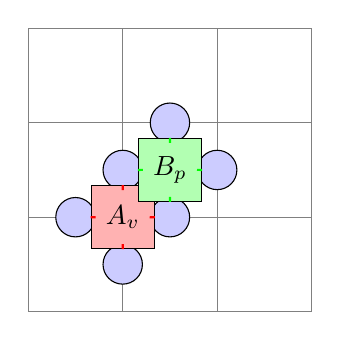
\begin{tikzpicture}[scale=1.2]
    \tikzstyle{dataq} = [circle, draw, fill=blue!20, inner sep=0pt, minimum size=5mm]
    \tikzstyle{vertexop} = [rectangle, draw, fill=red!30, inner sep=0pt, minimum size=8mm]
    \tikzstyle{plaqop} = [rectangle, draw, fill=green!30, inner sep=0pt, minimum size=8mm]

    % Grid structure
    \draw[gray, thin] (0,0) grid (3,3);

    % Data qubits
    \node[dataq] (q01v) at (1, 0.5) {};
    \node[dataq] (q10h) at (0.5, 1) {};
    \node[dataq] (q11v) at (1, 1.5) {};
    \node[dataq] (q11h) at (1.5, 1) {};
    \node[dataq] (q12h) at (1.5, 2) {};
    \node[dataq] (q21v) at (2, 1.5) {};

    % Stabilizers
    \node[vertexop] (A11) at (1,1) {$A_v$};
    \node[plaqop] (B11) at (1.5,1.5) {$B_p$};

    % Highlight stabilizers
    \draw[red, thick] (q01v) -- (A11);
    \draw[red, thick] (q10h) -- (A11);
    \draw[red, thick] (q11v) -- (A11);
    \draw[red, thick] (q11h) -- (A11);

    \draw[green, thick] (q11v) -- (B11);
    \draw[green, thick] (q11h) -- (B11);
    \draw[green, thick] (q12h) -- (B11);
    \draw[green, thick] (q21v) -- (B11);

\end{tikzpicture}
\caption{A section of the surface code lattice. Data qubits (blue circles) are on the edges. A \textbf{star operator} $A_v$ (red) is a product of $X$ operators on the four qubits meeting at a vertex $v$. A \textbf{plaquette operator} $B_p$ (green) is a product of $Z$ operators on the four qubits bounding a face $p$. Note that $A_v$ and $B_p$ share two qubits.}
\label{fig:surface_code_lattice}
\end{figure}

Like all stabilizer codes, the codespace is the simultaneous $+1$ eigenspace of all these stabilizers. For the surface code, the stabilizers are generated from two basic operators, as illustrated in Figure~\ref{fig:surface_code_lattice}:

\begin{itemize}
    \item \textbf{Star operators (Vertex operators):} For each vertex $v$ in the lattice (excluding boundaries for now), we define a star operator $A_v$ as the product of Pauli $X$ operators on all data qubits connected to that vertex.
    $$ A_v = \bigotimes_{i \in \text{star}(v)} X_i $$
    One way to try to remember that the vertex operators are products of $X$ operators is just tilting the cross gives you an $X$.

    \item \textbf{Plaquette operators (Face operators):} For each plaquette $p$ in the lattice, we define a plaquette operator $B_p$ as the product of Pauli $Z$ operators on all data qubits forming the boundary of that plaquette.
    $$ B_p = \bigotimes_{i \in \text{boundary}(p)} Z_i $$
    Another way of remembering this is that the faces on the surface code grid created "$Z$ones".
\end{itemize}

An essential property is that all these stabilizer operators commute.
\begin{itemize}
    \item $[A_v, A_{v'}]=0$ and $[B_p, B_{p'}]=0$. Two operators of the same type are either disjoint (acting on different qubits) or they overlap on some qubits.
    If they are not disjoint it doesn't matter either since $[X,X] = [Z,Z] = 0$.
    \item $[A_v, B_p]=0$. A star and a plaquette operator also always commute. They are either disjoint or, as shown in Figure~\ref{fig:surface_code_lattice}, they share exactly two qubits. Since Pauli operators commute if they have an even number of positions where they both anti-commute (e.g., an $X$ and a $Z$ on the same qubit), and here we have two such positions, the overall operators commute. For $A_v$ and $B_p$ in the figure, let the shared qubits be $q_a$ and $q_b$. Then $A_v = X_a X_b \dots$ and $B_p = Z_a Z_b \dots$. Their product is $(X_a X_b)(Z_a Z_b) = X_a Z_a X_b Z_b = (-Z_a X_a)(-Z_b X_b) = Z_a Z_b X_a X_b$. So they commute.
\end{itemize}

The stabilizers of the surface code are formed from all combinations of these two types of operators.

In this case we can make an observation about what combinations of these operators give us:

\begin{center}
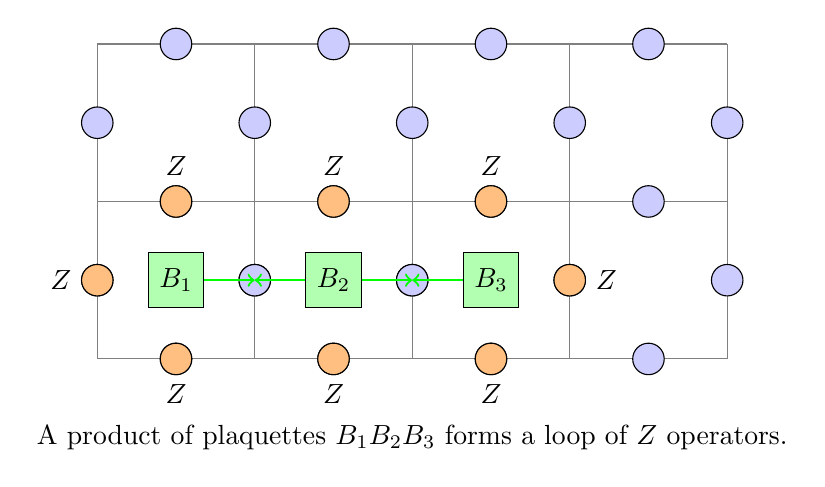
\begin{tikzpicture}[scale=2.0]
    \tikzstyle{dataq} = [circle, draw, fill=blue!20, inner sep=0pt, minimum size=4mm]
    \tikzstyle{plaqop} = [rectangle, draw, fill=green!30, inner sep=0pt, minimum size=7mm]

    % Grid
    \draw[step=1.0, gray, thin] (0,0) grid (4,2);

    % Data qubits
    \foreach \x in {0,...,4} \foreach \y in {0,...,2} {
        \ifnum\y<2 \node[dataq] at (\x, \y+0.5) {}; \fi
        \ifnum\x<4 \node[dataq] at (\x+0.5, \y) {}; \fi
    }

    % Plaquettes
    \node[plaqop] (p1) at (0.5,0.5) {$B_1$};
    \node[plaqop] (p2) at (1.5,0.5) {$B_2$};
    \node[plaqop] (p3) at (2.5,0.5) {$B_3$};

    % Data qubits for the B1 B2 B3 product - redraw with labels
    % Outer loop
    \node[dataq,label=below:$Z$,fill=orange!50] at (0.5,0) {};
    \node[dataq,label=below:$Z$,fill=orange!50] at (1.5,0) {};
    \node[dataq,label=below:$Z$,fill=orange!50] at (2.5,0) {};
    \node[dataq,label=above:$Z$,fill=orange!50] at (0.5,1) {};
    \node[dataq,label=above:$Z$,fill=orange!50] at (1.5,1) {};
    \node[dataq,label=above:$Z$,fill=orange!50] at (2.5,1) {};
    \node[dataq,label=left:$Z$,fill=orange!50] at (0,0.5) {};
    \node[dataq,label=right:$Z$,fill=orange!50] at (3,0.5) {};

    % Cancelled qubits
    \node[dataq] at (1,0.5) {}; % Cancelled B1-B2
    \node[dataq] at (2,0.5) {}; % Cancelled B2-B3

    % Arrows
    \draw[green, thick, ->] (p1) -- (1,0.5);
    \draw[green, thick, ->] (p2) -- (1,0.5);
    \draw[green, thick, ->] (p2) -- (2,0.5);
    \draw[green, thick, ->] (p3) -- (2,0.5);

    \node at (2, -0.5) {A product of plaquettes $B_1 B_2 B_3$ forms a loop of $Z$ operators.};
\end{tikzpicture}
\end{center}

Combinations/products of plaquette and vertex operators create loops in the surface code. 
So the entire set of stabilizers for the surface code are just sets of disjoint loops in the lattice.

\subsection{Error Detection and Syndromes}
We now have an understanding of the stabilizers for this code, but how does error detection work?
The state of the system is protected as long as it remains in the $+1$ eigenspace of all stabilizers. An error $E$ (a Pauli operator) is detected if it anti-commutes with at least one stabilizer $S$.

\begin{itemize}
    \item \textbf{Bit-flip ($X$) errors:} Suppose a bit-flip error $X_k$ occurs on a single data qubit $q_k$. This error operator $X_k$ commutes with all the star operators $A_v$ (since they are products of $X$'s). However, $q_k$ is on the boundary of two plaquettes, say $p_1$ and $p_2$. The error $X_k$ will anti-commute with the two corresponding plaquette operators, $B_{p_1}$ and $B_{p_2}$. Measuring these stabilizers will yield $-1$. We say that the error has created a pair of \textbf{$Z$-defects} (or \textbf{anyons}) on the plaquettes $p_1$ and $p_2$.

    \item \textbf{Phase-flip ($Z$) errors:} Suppose a phase-flip error $Z_k$ occurs on $q_k$. This error commutes with all plaquette operators $B_p$. However, the qubit $q_k$ connects two vertices, say $v_1$ and $v_2$. The error $Z_k$ will anti-commute with the two star operators $A_{v_1}$ and $A_{v_2}$. Measuring these stabilizers will yield $-1$, creating a pair of \textbf{$X$-defects} on vertices $v_1$ and $v_2$.

    \item \textbf{$Y$ errors:} A $Y_k$ error is equivalent to $iX_kZ_k$. It will anti-commute with the two adjacent star operators \textit{and} the two adjacent plaquette operators, creating both types of defects simultaneously.
\end{itemize}

\begin{example}[Detecting an $X$ Error]
Consider a single bit-flip error $X_k$ on a qubit $q_k$ in the lattice.
\begin{center}
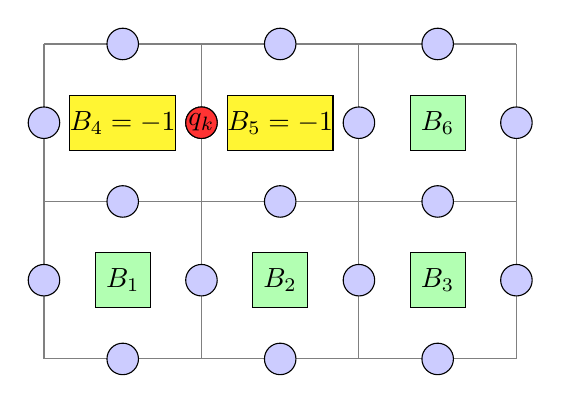
\begin{tikzpicture}[scale=2.0]
    \tikzstyle{dataq} = [circle, draw, fill=blue!20, inner sep=0pt, minimum size=4mm]
    \tikzstyle{plaqop} = [rectangle, draw, fill=green!30, inner sep=0pt, minimum size=7mm]
    \tikzstyle{defect} = [rectangle, draw, fill=yellow!80, inner sep=0pt, minimum size=7mm]

    % Grid
    \draw[step=1.0, gray, thin] (0,0) grid (3,2);

    % Data qubits
    \foreach \x in {0,...,3} \foreach \y in {0,...,2} {
        \ifnum\y<2 \node[dataq] at (\x, \y+0.5) {}; \fi
        \ifnum\x<3 \node[dataq] at (\x+0.5, \y) {}; \fi
    }
    % The error
    \node[dataq, fill=red!80] (err) at (1, 1.5) {}; 
    \node at (0.7, 1.5) {$X_k$}; \node at (1, 1.5) {$q_k$};

    % Plaquettes
    \node[plaqop] (p1) at (0.5,0.5) {$B_1$};
    \node[plaqop] (p2) at (1.5,0.5) {$B_2$};
    \node[plaqop] (p3) at (2.5,0.5) {$B_3$};
    \node[defect] (d1) at (0.5,1.5) {$B_4=-1$};
    \node[defect] (d2) at (1.5,1.5) {$B_5=-1$};
    \node[plaqop] (p6) at (2.5,1.5) {$B_6$};

\end{tikzpicture}
\end{center}
The error $X_k$ anti-commutes with the plaquette operators $B_4$ and $B_5$ because it is part of their definition. It commutes with all other plaquette operators since they act as the identity on $q_k$.
Therefore, measuring the plaquette stabilizers reveals a syndrome with value $-1$ at the locations of $B_4$ and $B_5$.
\end{example}

Errors occurring at neighboring qubits gives rise to \textbf{error chains}. In the above example, this was just an error chain of length 1 with $B_4$ and $B_5$ being the endpoints.
Let's examine a longer error chain, but first in the case of $Z$ errors (which are detected by vertex operators).

\begin{example}[$Z$ Error Chain]
A string of phase-flip ($Z$) errors will create a pair of $X$-defects at the vertices at the ends of the error chain. Consider a string of three adjacent phase-flip errors, $E = Z_a Z_b Z_c$.
The two star stabilizers at the ends of the chain will be violated, but the star stabilizers in the middle of the chain will not be,
because they anti-commute with \emph{two} of the error operators, leading to a $(-1) \times (-1) = +1$ overall factor.
The syndrome only reveals the endpoints.

\begin{center}
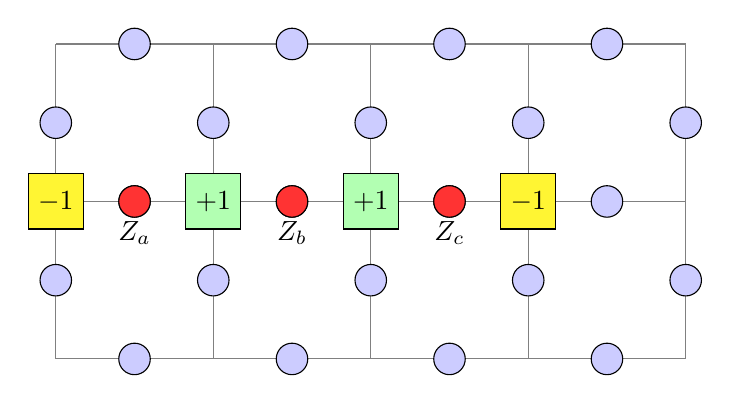
\begin{tikzpicture}[scale=2.0]
    \tikzstyle{dataq} = [circle, draw, fill=blue!20, inner sep=0pt, minimum size=4mm]
    \tikzstyle{vertexop} = [rectangle, draw, fill=green!30, inner sep=0pt, minimum size=7mm]
    \tikzstyle{defect} = [rectangle, draw, fill=yellow!80, inner sep=0pt, minimum size=7mm]

    % Grid
    \draw[step=1.0, gray, thin] (0,0) grid (4,2);

    % Data qubits
    \foreach \x in {0,...,4} \foreach \y in {0,...,2} {
        \ifnum\y<2 \node[dataq] at (\x, \y+0.5) {}; \fi
        \ifnum\x<4 \node[dataq] at (\x+0.5, \y) {}; \fi
    }
    % The error chain
    \node[dataq, fill=red!80] (err1) at (0.5, 1) {};
    \node[dataq, fill=red!80] (err2) at (1.5, 1) {};
    \node[dataq, fill=red!80] (err3) at (2.5, 1) {};
    \node at (0.5, 0.8) {$Z_a$};
    \node at (1.5, 0.8) {$Z_b$};
    \node at (2.5, 0.8) {$Z_c$};


    % Vertices
    \node[defect] (v1) at (0,1) {$-1$};
    \node[vertexop] (v2) at (1,1) {$+1$};
    \node[vertexop] (v3) at (2,1) {$+1$};
    \node[defect] (v4) at (3,1) {$-1$};

\end{tikzpicture}
\end{center}
The error chain $Z_a Z_b Z_c$ creates defects only on the vertices at the ends of the chain. The vertices in the middle are unaffected because they are connected to two errors.
\end{example}

\begin{example}[$X$ Error Chain]
Now let's examine a length 3 $X$ error chain.
\begin{center}
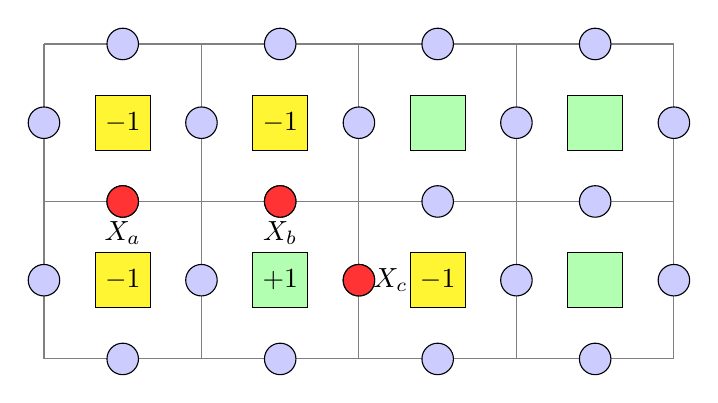
\begin{tikzpicture}[scale=2.0]
    \tikzstyle{dataq} = [circle, draw, fill=blue!20, inner sep=0pt, minimum size=4mm]
    \tikzstyle{plaqop} = [rectangle, draw, fill=green!30, inner sep=0pt, minimum size=7mm]
    \tikzstyle{defect} = [rectangle, draw, fill=yellow!80, inner sep=0pt, minimum size=7mm]

    % Grid
    \draw[step=1.0, gray, thin] (0,0) grid (4,2);

    % Data qubits
    \foreach \x in {0,...,4} \foreach \y in {0,...,2} {
        \ifnum\y<2 \node[dataq] at (\x, \y+0.5) {}; \fi
        \ifnum\x<4 \node[dataq] at (\x+0.5, \y) {}; \fi
    }
    % The error chain
    \node[dataq, fill=red!80] (err1) at (0.5, 1) {};
    \node[dataq, fill=red!80] (err2) at (1.5, 1) {};
    \node[dataq, fill=red!80] (err3) at (2, 0.5) {};
    \node at (0.5, 0.8) {$X_a$};
    \node at (1.5, 0.8) {$X_b$};
    \node at (2.2, 0.5) {$X_c$};


    % Plaquettes
    \node[defect] (p1) at (0.5,0.5) {$-1$};
    \node[plaqop] (p2) at (1.5,0.5) {$+1$};
    \node[defect] (p3) at (2.5,0.5) {$-1$};
    \node[plaqop] (p4) at (3.5,0.5) {};
    \node[defect] (d1) at (0.5,1.5) {$-1$};
    \node[defect] (p5) at (1.5,1.5) {$-1$};
    \node[plaqop] (d2) at (2.5,1.5) {};
    \node[plaqop] (p6) at (3.5,1.5) {};

\end{tikzpicture}
\end{center}
This doesn't show the nice endpoint property that we saw above with the $Z$ error chain.
Luckily for us, with a shift of perspective it actually does. This shift of perspective is called the \textbf{dual lattice}.
\end{example}

\subsection{The Dual Lattice}

The asymmetry between how we visualize $X$ and $Z$ error chains can be resolved by introducing the \textbf{dual lattice}.
The dual lattice can be thought of as the original (primal) grid shifted down and to the right.
More formally, it is constructed by placing a vertex at the center of each plaquette of the original grid, and connecting these new vertices if the corresponding plaquettes share a data qubit.

\begin{itemize}
    \item The vertex operators of the dual lattice correspond to the plaquettes (Z-stabilizers) of the primal grid.
    \item The plaquette operators of the dual lattice correspond to the vertex operators on the primal grid.
    \item Data qubits remain edges, but their orientations are rotated 90 degrees.
\end{itemize}

\begin{center}
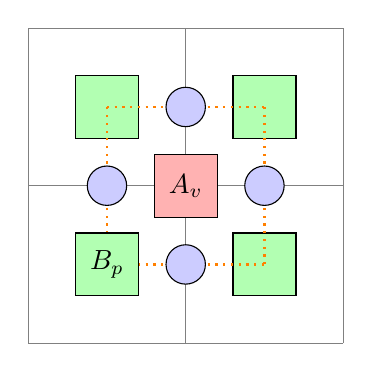
\begin{tikzpicture}[scale=2.0]
    \tikzstyle{dataq} = [circle, draw, fill=blue!20, inner sep=0pt, minimum size=5mm]
    \tikzstyle{vertexop} = [rectangle, draw, fill=red!30, inner sep=0pt, minimum size=8mm]
    \tikzstyle{plaqop} = [rectangle, draw, fill=green!30, inner sep=0pt, minimum size=8mm]
    \tikzstyle{dualvertex} = [circle, draw, fill=orange!50, inner sep=0pt, minimum size=4mm]

    % Primal Grid
    \draw[gray, thin] (0,0) grid (2,2);

    % Dual Grid
    \foreach \x in {0,...,1} \foreach \y in {0,...,1} {
        \node[plaqop] at (\x+0.5, \y+0.5) {};
    }
    \draw[orange, dotted, thick] (0.5,0.5) -- (1.5,0.5);
    \draw[orange, dotted, thick] (0.5,1.5) -- (1.5,1.5);
    \draw[orange, dotted, thick] (0.5,0.5) -- (0.5,1.5);
    \draw[orange, dotted, thick] (1.5,0.5) -- (1.5,1.5);

    % Data qubits
    \node[dataq] at (1, 0.5) {};
    \node[dataq] at (0.5, 1) {};
    \node[dataq] at (1.5, 1) {};
    \node[dataq] at (1, 1.5) {};

    % Stabilizers
    \node[vertexop] (A11) at (1,1) {$A_v$};
    \node[plaqop] (B11) at (0.5,0.5) {$B_p$};
\end{tikzpicture}
\end{center}

With this perspective, an $X$ error on a data qubit now is caught by the dual-lattice $Z$ vertex operators.

This means that the chain of $X$ errors on the primal grid (that we saw above) becomes a chain of errors on the dual lattice, creating defects only at the endpoints of the chain.

\begin{example}[$X$ Error Chain in the Dual Lattice]
Let's visualize the same L-shaped $X$ error chain from the previous example on the dual lattice. The primal lattice is in gray, with data qubits as blue circles. The dual lattice is overlaid in orange. An error chain of three $X$ operators ($X_a, X_b, X_c$) is shown on the red data qubits.

\begin{center}
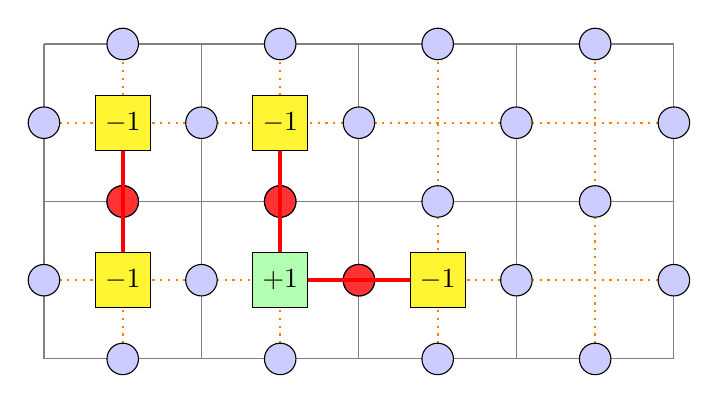
\begin{tikzpicture}[scale=2.0]
    \tikzstyle{dataq} = [circle, draw, fill=blue!20, inner sep=0pt, minimum size=4mm]
    \tikzstyle{plaqop} = [rectangle, draw, fill=green!30, inner sep=0pt, minimum size=7mm]
    \tikzstyle{defect} = [rectangle, draw, fill=yellow!80, inner sep=0pt, minimum size=7mm]
    \tikzstyle{dualvertex} = [circle, draw, fill=orange!50, inner sep=0pt, minimum size=4mm]

    % Primal Grid
    \draw[step=1.0, gray, thin] (0,0) grid (4,2);

    % Dual Grid
    % \foreach \x in {0,...,3} \foreach \y in {0,...,1} {
    %     \node[dualvertex] at (\x+0.5, \y+0.5) {};
    % }
    \foreach \x in {-0.5,...,2.5} \foreach \y in {0,...,1} {
        \draw[orange, dotted, thick] (\x+0.5, \y+0.5) -- (\x+1.5, \y+0.5);
    }
    \foreach \x in {0,...,3} \foreach \y in {0,...,0} {
        \draw[orange, dotted, thick] (\x+0.5, \y) -- (\x+0.5, \y+2);
    }

    % Data qubits
    \foreach \x in {0,...,4} \foreach \y in {0,...,2} {
        \ifnum\y<2 \node[dataq] at (\x, \y+0.5) {}; \fi
        \ifnum\x<4 \node[dataq] at (\x+0.5, \y) {}; \fi
    }
    
    % The error chain
    \node[dataq, fill=red!80] (err1) at (0.5, 1) {};
    \node[dataq, fill=red!80] (err2) at (1.5, 1) {};
    \node[dataq, fill=red!80] (err3) at (2, 0.5) {};

    % Draw the error path on the dual grid
    \draw[red, ultra thick] (0.5,0.5) -- (0.5,1.5);
    \draw[red, ultra thick] (1.5,0.5) -- (1.5,1.5);
    \draw[red, ultra thick] (1.5,0.5) -- (2.5,0.5);

    % Defects
    \node[defect] at (0.5,0.5) {$-1$};
    \node[defect] at (0.5,1.5) {$-1$};
    \node[plaqop] at (1.5,0.5) {$+1$};
    \node[defect] at (1.5,1.5) {$-1$};
    \node[defect] at (2.5,0.5) {$-1$};
\end{tikzpicture}
\end{center}

The $X$ error chain now appears as two error chains in the dual view! Each chain having the expected detection events at its endpoints.
\end{example}

\subsection{Correcting Surface Code Errors}

We now have some understanding around detection events, but \emph{how do we actually correct errors}? 
For example we know that errors create excitations (defects)
that with the right view are just endpoints of some string. There could be \emph{many} such strings with the same endpoints.

\begin{center}
How do we know which path was the right path?
\end{center}

Going back to the task at hand of decoding, we know that if there are multiple paths from one endpoint to another, a pair of such paths makes a \textbf{loop}.

So let $E_{true}$ be the real error that resulted in a detection event (defects) $A$ and $B$. 
If we instead choose the path $E_{guess}$ (which also results in detection events $A$ and $B$) then
we get a loop from $A$ to $B$ traversing $E_{true}$ and then traversing $E_{guess}$ backwards (since Pauli operators are their own inverse direction doesn't actually matter).
In the event that this is a trivial error (we will get to what this means), that just means this
is a stabilizer!

So then $E_{guess}^\dagger E_{true} |\psi\rangle$ would be our final corrected state, but $E_{guess}^\dagger E_{true}$ is just a stabilizer operation on a codeword. So we get back our starting state $|\psi\rangle$.

\subsection{Surface Codes Actual Lattices}

We now need to address what we meant by \textbf{trivial} errors. These are just loops that are stabilizers. But aren't all loops stabilizers?
This answer depends on whether we are using a \textbf{Planar} surface code or a \textbf{Toric} surface code. The difference between these two are that
a planar surface code is a lattice that you can write on a flat sheet of paper which looks specifically like:

\begin{center}
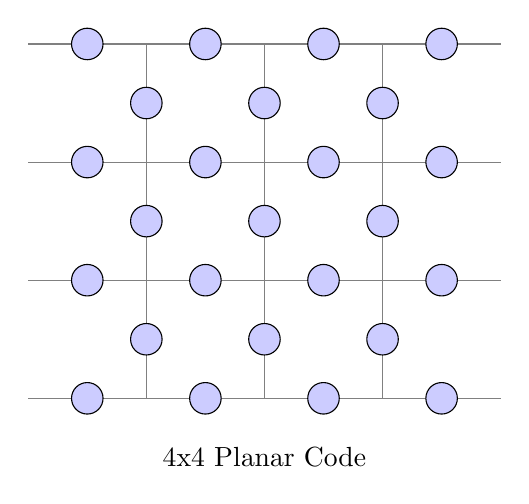
\begin{tikzpicture}[scale=1.5]
    \tikzstyle{dataq} = [circle, draw, fill=blue!20, inner sep=0pt, minimum size=4mm]

    % Draw grid lines
    
    % Draw all horizontal lines (from y=0 to y=4)
    \foreach \y in {0,...,3} {
        \draw[gray, thin] (0,\y) -- (4,\y);
    }
    
    % Draw only the inner vertical lines (from x=1 to x=3)
    % This skips the outer lines at x=0 and x=4
    \foreach \x in {1,...,3} {
        \draw[gray, thin] (\x,0) -- (\x,3);
    }

    % Horizontal data qubits
    \foreach \y in {0,...,3} {
        \foreach \x in {0,...,3} {
            \node[dataq] at (\x+0.5, \y) {};
        }
    }
    % Vertical data qubits (not on left/right boundaries)
    \foreach \y in {0,...,2} {
        \foreach \x in {1,...,3} {
            \node[dataq] at (\x, \y+0.5) {};
        }
    }
    \node at (2, -0.5) {4x4 Planar Code};
\end{tikzpicture}
\end{center}

The toric code on the other hand has periodic boundary conditions meaning that its vertical sides connect to each other and its horizontal sides connect to one another.
It exists in 3 dimensions, and if you aren't familiar with a Torus then you may be familiar with a donut. Written out in 2 dimensions it looks like:

\begin{center}
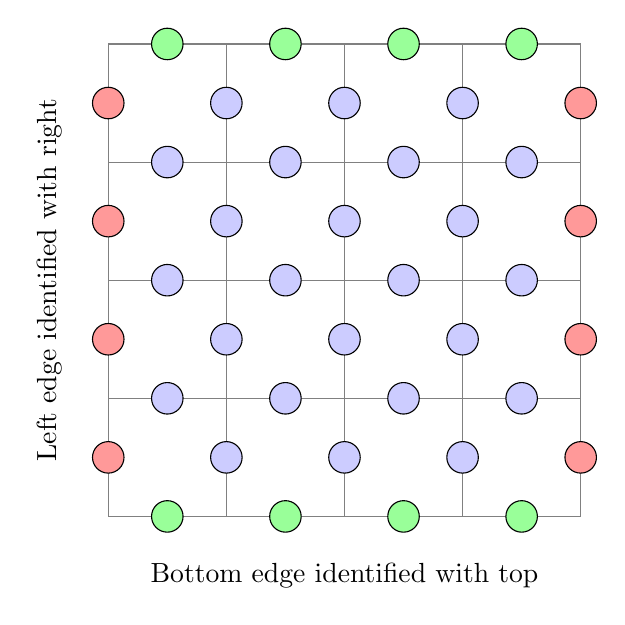
\begin{tikzpicture}[scale=1.5]
    \def\d{4}
    
    % --- DEFINE STYLES ---
    % Style for bulk qubits
    \tikzstyle{dataq} = [circle, draw, fill=blue!20, inner sep=0pt, minimum size=4mm]
    % Style for horizontal (top/bottom) boundary qubits
    \tikzstyle{h_boundary_q} = [dataq, fill=green!40]
    % Style for vertical (left/right) boundary qubits
    \tikzstyle{v_boundary_q} = [dataq, fill=red!40]

    % Draw grid
    \draw[gray, thin] (0,0) grid (\d,\d);

    % --- DRAW QUBITS WITH CONDITIONAL STYLING ---

    % 1. Data qubits on horizontal lines (y=0, 1, 2, 3, 4)
    \foreach \y in {0,...,\d} {
        \foreach \x in {0,...,3} {
            % Check if y is on the top or bottom boundary
            \ifnum\y=0 \def\style{h_boundary_q}
            \else
                \ifnum\y=\d \def\style{h_boundary_q}
                \else \def\style{dataq}
                \fi
            \fi
            % Draw the node with the chosen style
            \node[\style] at (\x+0.5, \y) {};
        }
    }
    
    % 2. Data qubits on vertical lines (x=0, 1, 2, 3, 4)
    \foreach \x in {0,...,\d} {
        \foreach \y in {0,...,3} {
            % Check if x is on the left or right boundary
            \ifnum\x=0 \def\style{v_boundary_q}
            \else
                \ifnum\x=\d \def\style{v_boundary_q}
                \else \def\style{dataq}
                \fi
            \fi
            % Draw the node with the chosen style
            \node[\style] at (\x, \y+0.5) {};
        }
    }

    % Identification labels
    \node at (\d/2, -0.5) {Bottom edge identified with top};
    \node[rotate=90] at (-0.5, \d/2) {Left edge identified with right};
\end{tikzpicture}
\end{center}

Now that we have these two grids in mind, let's focus on the Toric code since it is the most common. We need to address what we mean by trivial errors.
We know that if an error occurs and the loop that comes from it is a stabilizer operator then we are good.

\begin{center}
Do all loops result in a stabilizer?
\end{center}

This leads us to the next important concept. What are the logical operators of the surface code?

\subsection{Logical Qubits and Operators}

We know that logical operators have to commute with our stabilizers, but cannot be part of the stabilizer set so that it causes a nontrivial operation on the codespace.

The logical operator is then essentially an error that is undetectable.

\begin{center}
    What errors would be undetectable by the toric code?
\end{center}

We know that strings of errors have endpoints, what would happen if these endpoints collided with each other?

\begin{itemize}
    \item \textbf{Logical Z operators ($\bar{Z}_{\rightarrow, \uparrow}$):} A logical $Z$ operator is a string of single-qubit $Z$ operators that stretches around one side of the torus (and squashes its endpoints).
    \begin{center}
        \begin{minipage}{.5\textwidth}
            \centering
            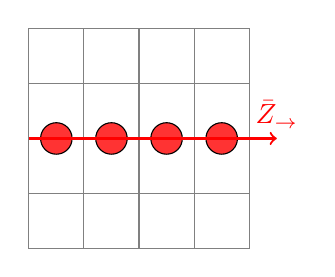
\begin{tikzpicture}[scale=0.7]
                \tikzstyle{dataq} = [circle, draw, fill=blue!20, inner sep=0pt, minimum size=4mm]
                \draw[step=1.0, gray, thin] (0,0) grid (4,4);
                \foreach \x in {0,...,3} {
                    \node[dataq, fill=red!80] at (\x+0.5, 2) {};
                }
                \draw[red, thick, ->] (0, 2) -- (4.5, 2) node[above] {$\bar{Z}_\rightarrow$};
            \end{tikzpicture}
        \end{minipage}%
        \begin{minipage}{.5\textwidth}
            \centering
            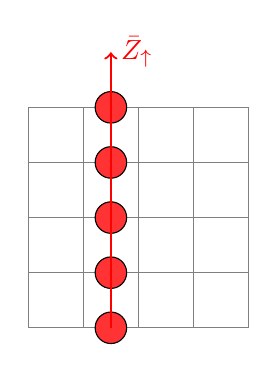
\begin{tikzpicture}[scale=0.7]
                \tikzstyle{dataq} = [circle, draw, fill=blue!20, inner sep=0pt, minimum size=4mm]
                \draw[step=1.0, gray, thin] (0,0) grid (4,4);
                \foreach \y in {0,...,4} {
                    \node[dataq, fill=red!80] at (1.5, \y) {};
                }
                \draw[red, thick, ->] (1.5, 0) -- (1.5, 5) node[right] {$\bar{Z}_\uparrow$};
            \end{tikzpicture}
        \end{minipage}
    \end{center}
    This operator $\bar{Z}$ commutes with all star stabilizers $A_v$ because they overlap on 0 or 2 qubits. It also commutes with all plaquette stabilizers since Pauli operators commute with themselves.
    However, it is not a product of stabilizers, so it is non-trivial on the codespace.

    \item \textbf{Logical X operators ($\bar{X}_{\rightarrow, \uparrow}$):} Similarly, a logical $X$ operator is a string of single-qubit $X$ operators that stretch vertically, but are on horizontal edge data qubits, or stretches horizontally on vertical edge qubits.
    Remember that this is an error string in the dual lattice that wraps around the Torus.
    \begin{center}
        \begin{minipage}{.5\textwidth}
            \centering
            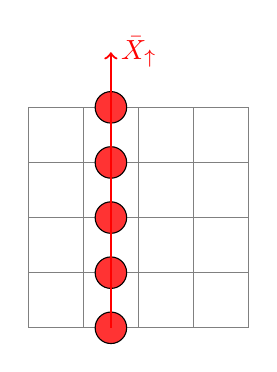
\begin{tikzpicture}[scale=0.7]
                \tikzstyle{dataq} = [circle, draw, fill=blue!20, inner sep=0pt, minimum size=4mm]
                \draw[step=1.0, gray, thin] (0,0) grid (4,4);
                \foreach \y in {0,...,4} {
                    \node[dataq, fill=red!80] at (1.5, \y) {};
                }
                \draw[red, thick, ->] (1.5, 0) -- (1.5, 5) node[right] {$\bar{X}_\uparrow$};
            \end{tikzpicture}
        \end{minipage}%
        \begin{minipage}{.5\textwidth}
            \centering
            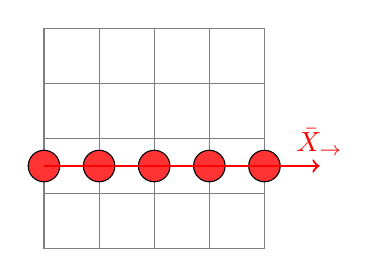
\begin{tikzpicture}[scale=0.7]
                \tikzstyle{dataq} = [circle, draw, fill=blue!20, inner sep=0pt, minimum size=4mm]
                \draw[step=1.0, gray, thin] (0,0) grid (4,4);
                \foreach \x in {0,...,4} {
                    \node[dataq, fill=red!80] at (\x, 1.5) {};
                }
                \draw[red, thick, ->] (0, 1.5) -- (5, 1.5) node[above] {$\bar{X}_\rightarrow$};
            \end{tikzpicture}
        \end{minipage}
    \end{center}
    This operator $\bar{X}$ commutes with all stabilizers for the same reasons.
\end{itemize}

Crucially, the logical $\bar{X}$ and logical $\bar{Z}$ operators anti-commute since they overlap only on a single qubit.

You may ask, don't we have multiple options for these logical operators? For example we can choose any row to be the logical $Z_\rightarrow$ operator.
That is true, but luckily these can actually be \emph{deformed} into one another. For example to change logical $Z$ row into another, we can just apply the plaquette operators in between them.
The vertical edges cancel out, and you are left with the logical $Z$ operator on a different row. This also makes sense mathematically because for a stabilizer $S$ we have:
$$\overline{Z} \cdot S |\psi\rangle = \overline{Z} |\psi\rangle$$
So technically $\overline{Z} \cdot S$ is also a logical operator. We just make a choice as a \emph{convention}.

The toric code gives us two distinct logical $Z$ operators and logical $X$ operators, and so in total we get two logical qubits from it. Let's do a quick count of the Hilbert space.

\subsubsection{Toric Code Counting}
If we have $L\times L$ many squares in our lattice, that gives us $(L+1)L$ many horizontal edges and $(L+1)(L)$ many vertical edges so $2(L^2 + L)$ many qubits total... but wait we have actually glued the boundaries together.
So we must remove $L$ many qubits from \emph{one} vertical side and $L$ from \emph{one} horizontal side leaving us with $2L^2$ many qubits. $2L^2$ many qubits gives us a total Hilbert space of dimension $2^{2L^2}$.

\begin{figure}[h!]
\centering
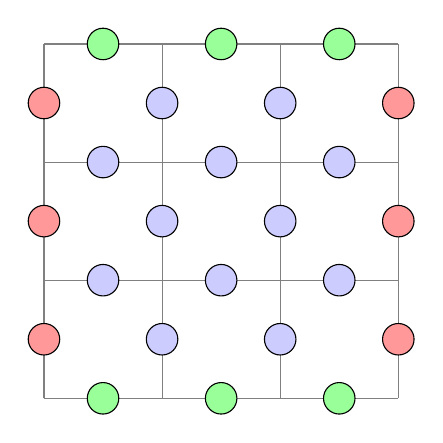
\begin{tikzpicture}[scale=1.5]
    \def\d{3}
    
    % --- DEFINE STYLES ---
    % Style for bulk qubits
    \tikzstyle{dataq} = [circle, draw, fill=blue!20, inner sep=0pt, minimum size=4mm]
    % Style for horizontal (top/bottom) boundary qubits
    \tikzstyle{h_boundary_q} = [dataq, fill=green!40]
    % Style for vertical (left/right) boundary qubits
    \tikzstyle{v_boundary_q} = [dataq, fill=red!40]

    % Draw grid
    \draw[gray, thin] (0,0) grid (\d,\d);

    % --- DRAW QUBITS WITH CONDITIONAL STYLING ---

    % 1. Data qubits on horizontal lines (y=0, 1, 2, 3, 4)
    \foreach \y in {0,...,\d} {
        \foreach \x in {0,...,2} {
            % Check if y is on the top or bottom boundary
            \ifnum\y=0 \def\style{h_boundary_q}
            \else
                \ifnum\y=\d \def\style{h_boundary_q}
                \else \def\style{dataq}
                \fi
            \fi
            % Draw the node with the chosen style
            \node[\style] at (\x+0.5, \y) {};
        }
    }
    
    % 2. Data qubits on vertical lines (x=0, 1, 2, 3, 4)
    \foreach \x in {0,...,\d} {
        \foreach \y in {0,...,2} {
            % Check if x is on the left or right boundary
            \ifnum\x=0 \def\style{v_boundary_q}
            \else
                \ifnum\x=\d \def\style{v_boundary_q}
                \else \def\style{dataq}
                \fi
            \fi
            % Draw the node with the chosen style
            \node[\style] at (\x, \y+0.5) {};
        }
    }

    % Identification labels
\end{tikzpicture}
\caption{$L=3$ Toric Code}
\end{figure}

Now how many stabilizers do we have? Well, we have $L^2$ many plaquette operators for the $L\times L$ lattice. For the vertex operators we have to count how many unique vertices that we have.

We first notice that neighboring faces will have most of their vertices overcounted, so let's just identify the top left vertex to each face, this one is actually never double counted. This gives us exactly $L^2$ many vertex operators too.

So we should get $2L^2$ many generators, except for the fact that this is not an independent set, for instance the top left plaquette operator could be generated by using the remaining plaquettes.
This fact leaves us with $2L^2 - 2$ many independent stabilizer generators (we must leave out one plaquette and one vertex), each one halving the overall Hilbert space (combinations formed from them don't reduce the Hilbert space any further since any stabilizer, $S_3$, generated by say $S_1,S_2$ has the same eigenspace as the shared eigenspace of $S_1$ \& $S_2$ (prove it!)).
Hence we are left with a Hilbert space of size $2^2$, so two logical qubits exactly!

The \textbf{code distance} $d$ of the surface code is the size of the smallest (lowest weight) logical operator.
For a $L \times L$ lattice, the shortest path between two opposite boundaries is of length $L$. Therefore, the code distance is $L$.
This means the code can correct up to $t = \lfloor(L-1)/2\rfloor$ errors. To increase the protection, we simply need to build a larger lattice.
This scalability is a major advantage of the surface code.

Thus, for the $L\times L$ Toric code we have a $(2L^2,2,L)$ code which can correct up to $\lfloor(L-1)/2\rfloor$ many errors!

\subsection{Decoding the Surface Code}

We have now shown that we can detect errors up to size $L$ for the $L\times L$ toric code, but how does this typically work?
Since errors create pairs of defects within the lattice, the \textbf{decoding} algorithm tries to pair up the detection events
in the \textbf{most likely} way. For instance if we have detection events $A,B,C,D$ and $A$ and $B$ are significantly close to one another in the lattice,
and so are $C$ and $D$, then it is much more likely that these events are paired (depending on your error probability model of course).

A popular decoding algorithm is \textbf{minimum weight perfect matching}, what this algorithm aims to do is to look at the set of defects and simply find the matching of defects that produces the minimum weight.
Typically the weight of a matching is defined to be the (inverse) likelihood of seeing that matching, i.e., figuring out how likely the path between the detection events is to occur. 
So finding the minimum weight perfect matching here gives you the \emph{most likely} configuration of errors that could explain the observed detection events.

\appendix
\section{Proof of the No-Cloning Theorem}
\label{sec:no_cloning}

The no-cloning theorem states that it is impossible to create an identical copy of an arbitrary unknown quantum state. Here we provide a proof by contradiction.

Assume there exists a unitary operator $U$ that can clone an arbitrary quantum state $|\psi\rangle$. The cloning process can be represented as:
$$ U(|\psi\rangle \otimes |s\rangle) = |\psi\rangle \otimes |\psi\rangle $$
where $|\psi\rangle$ is the state to be cloned, and $|s\rangle$ is some initial "blank" state.

Let's consider two different quantum states, $|\psi\rangle$ and $|\phi\rangle$. The cloning operation for these states would be:
\begin{align*}
    U(|\psi\rangle \otimes |s\rangle) &= |\psi\rangle \otimes |\psi\rangle \\
    U(|\phi\rangle \otimes |s\rangle) &= |\phi\rangle \otimes |\phi\rangle
\end{align*}

Now, let's take the inner product of these two equations. Since $U$ is a unitary operator, it preserves the inner product:
$$ \langle (U(|\psi\rangle \otimes |s\rangle)) | (U(|\phi\rangle \otimes |s\rangle)) \rangle = \langle (\psi\psi) | (\phi\phi) \rangle = (\langle\psi|\phi\rangle)^2 $$
The left side of the equation is:
$$ \langle (\psi s) | U^\dagger U | (\phi s) \rangle = \langle \psi s | \phi s \rangle = \langle\psi|\phi\rangle \langle s|s \rangle = \langle\psi|\phi\rangle $$
So we have the condition that for any two states $|\psi\rangle$ and $|\phi\rangle$, we must have:
$$ \langle\psi|\phi\rangle = (\langle\psi|\phi\rangle)^2 $$
This equation is only true if $\langle\psi|\phi\rangle = 0$ or $\langle\psi|\phi\rangle = 1$. This means the cloning machine would only work for states that are orthogonal or identical.

However, an arbitrary quantum state can be a superposition of other states. Let's consider a state $|\chi\rangle = \frac{1}{\sqrt{2}}(|\psi\rangle + |\phi\rangle)$, where $|\psi\rangle$ and $|\phi\rangle$ are orthogonal.
If we apply the cloning operator $U$ to $|\chi\rangle$, we get:
$$ U(|\chi\rangle \otimes |s\rangle) = \frac{1}{\sqrt{2}} (U(|\psi\rangle \otimes |s\rangle) + U(|\phi\rangle \otimes |s\rangle)) = \frac{1}{\sqrt{2}} (|\psi\rangle \otimes |\psi\rangle + |\phi\rangle \otimes |\phi\rangle) $$
But if the cloning were successful, we would expect to get:
$$ |\chi\rangle \otimes |\chi\rangle = \frac{1}{2} (|\psi\rangle + |\phi\rangle) \otimes (|\psi\rangle + |\phi\rangle) = \frac{1}{2} (|\psi\psi\rangle + |\psi\phi\rangle + |\phi\psi\rangle + |\phi\phi\rangle) $$
These two resulting states are not the same. This gives us the contradiction.

\section{Proof of Commuting Observables Theorem}
\label{sec:commuting_proof}

Here we prove that if two oberservables (hermitian and thus diagonalizable), $A$ and $B$, commute ($AB=BA$), they share a common basis of eigenvectors.

Let $|\psi\rangle$ be an eigenvector of $A$ with eigenvalue $\lambda$. So, $A|\psi\rangle = \lambda|\psi\rangle$.
Now, consider the vector $B|\psi\rangle$. Let's see how $A$ acts on it:
$$ A(B|\psi\rangle) = (AB)|\psi\rangle = (BA)|\psi\rangle = B(A|\psi\rangle) = B(\lambda|\psi\rangle) = \lambda(B|\psi\rangle) $$
This shows that $B|\psi\rangle$ is also an eigenvector of $A$ with the same eigenvalue $\lambda$.

\paragraph{Case 1: Non-degenerate eigenvalues}
If the eigenspace of $A$ for the eigenvalue $\lambda$ is one-dimensional (non-degenerate), then any eigenvector of $A$ with eigenvalue $\lambda$ must be a scalar multiple of $|\psi\rangle$.
Since $B|\psi\rangle$ is an eigenvector of $A$ with the same eigenvalue, it must be that $B|\psi\rangle = \mu|\psi\rangle$ for some scalar $\mu$.
This means that $|\psi\rangle$ is also an eigenvector of $B$ with eigenvalue $\mu$.
Thus, for non-degenerate eigenvalues of $A$, every eigenvector of $A$ is also an eigenvector of $B$.

\paragraph{Case 2: Degenerate eigenvalues}
If the eigenspace of $A$ for the eigenvalue $\lambda$, let's call it $V_\lambda$, is degenerate (i.e., has repeated eigenvalues so that the dimension of the space is more than 1), then for any vector $|v\rangle \in V_\lambda$, we have $A|v\rangle = \lambda|v\rangle$.

We have shown that $A(B|v\rangle) = \lambda(B|v\rangle)$, which means that if $|v\rangle \in V_\lambda$, then $B|v\rangle$ is also in $V_\lambda$. Thus, the eigenspace $V_\lambda$ is an \textbf{invariant subspace} under the action of $B$ (it maps the eigenspace to itself).

We can now consider the action of $B$ restricted to this subspace, an operator we can call $B|_{V_\lambda}$. Because we assume $A$ and $B$ are diagaonalizable (they are observables), the restriction $B|_{V_\lambda}$ is also diagonalizable within the subspace $V_\lambda$.

This diagonalizability \emph{guarantees} that we can find an orthonormal basis for $V_\lambda$ composed entirely of eigenvectors of $B$. Let $\{|\phi_i\rangle\}$ be such a basis.

For any vector $|\phi_i\rangle$ in this basis, two conditions hold:
\begin{enumerate}
    \item $A|\phi_i\rangle = \lambda|\phi_i\rangle$ (since $|\phi_i\rangle \in V_\lambda$)
    \item $B|\phi_i\rangle = \mu_i|\phi_i\rangle$ (since it is an eigenvector of $B$, with some eigenvalue $\mu_i$)
\end{enumerate}
Thus, every vector in this basis for $V_\lambda$ is a simultaneous eigenvector of both $A$ and $B$.

By finding such a basis for all eigenspaces of $A$ (both degenerate and non-degenerate), we can construct a complete basis for the entire Hilbert space consisting of simultaneous eigenvectors.

\end{document}
